% This LaTeX document needs to be compiled with XeLaTeX.
\documentclass[
  10
]{article}
\usepackage[margin=2cm,includehead=true,includefoot=true,centering,]{geometry}
\usepackage{xcolor}
\usepackage{ucharclasses}
\usepackage{hyperref}
\usepackage{amsmath,amssymb}
\usepackage{amsfonts}
\usepackage[version=4]{mhchem}
\usepackage{stmaryrd}
\usepackage{bbold}
\usepackage{polyglossia}
\usepackage{fontspec}
\usepackage{ctex}
\usepackage[export]{adjustbox}
\usepackage{tabularx}
\usepackage{booktabs}

\usepackage{setspace}
\setstretch{1.2}

\makeatletter
\@ifundefined{KOMAClassName}{% if non-KOMA class
  \IfFileExists{parskip.sty}{%
    \usepackage{parskip}
  }{% else
    \setlength{\parindent}{0pt}
    \setlength{\parskip}{6pt plus 2pt minus 1pt}}
}{% if KOMA class
  \KOMAoptions{parskip=half}}
\makeatother
\usepackage{color}
\usepackage{fancyvrb}
\newcommand{\VerbBar}{|}
\newcommand{\VERB}{\Verb[commandchars=\\\{\}]}
\DefineVerbatimEnvironment{Highlighting}{Verbatim}{commandchars=\\\{\}}
% Add ',fontsize=\small' for more characters per line
\newenvironment{Shaded}{}{}
\newcommand{\AlertTok}[1]{\textcolor[rgb]{1.00,0.00,0.00}{\textbf{#1}}}
\newcommand{\AnnotationTok}[1]{\textcolor[rgb]{0.38,0.63,0.69}{\textbf{\textit{#1}}}}
\newcommand{\AttributeTok}[1]{\textcolor[rgb]{0.49,0.56,0.16}{#1}}
\newcommand{\BaseNTok}[1]{\textcolor[rgb]{0.25,0.63,0.44}{#1}}
\newcommand{\BuiltInTok}[1]{\textcolor[rgb]{0.00,0.50,0.00}{#1}}
\newcommand{\CharTok}[1]{\textcolor[rgb]{0.25,0.44,0.63}{#1}}
\newcommand{\CommentTok}[1]{\textcolor[rgb]{0.38,0.63,0.69}{\textit{#1}}}
\newcommand{\CommentVarTok}[1]{\textcolor[rgb]{0.38,0.63,0.69}{\textbf{\textit{#1}}}}
\newcommand{\ConstantTok}[1]{\textcolor[rgb]{0.53,0.00,0.00}{#1}}
\newcommand{\ControlFlowTok}[1]{\textcolor[rgb]{0.00,0.44,0.13}{\textbf{#1}}}
\newcommand{\DataTypeTok}[1]{\textcolor[rgb]{0.56,0.13,0.00}{#1}}
\newcommand{\DecValTok}[1]{\textcolor[rgb]{0.25,0.63,0.44}{#1}}
\newcommand{\DocumentationTok}[1]{\textcolor[rgb]{0.73,0.13,0.13}{\textit{#1}}}
\newcommand{\ErrorTok}[1]{\textcolor[rgb]{1.00,0.00,0.00}{\textbf{#1}}}
\newcommand{\ExtensionTok}[1]{#1}
\newcommand{\FloatTok}[1]{\textcolor[rgb]{0.25,0.63,0.44}{#1}}
\newcommand{\FunctionTok}[1]{\textcolor[rgb]{0.02,0.16,0.49}{#1}}
\newcommand{\ImportTok}[1]{\textcolor[rgb]{0.00,0.50,0.00}{\textbf{#1}}}
\newcommand{\InformationTok}[1]{\textcolor[rgb]{0.38,0.63,0.69}{\textbf{\textit{#1}}}}
\newcommand{\KeywordTok}[1]{\textcolor[rgb]{0.00,0.44,0.13}{\textbf{#1}}}
\newcommand{\NormalTok}[1]{#1}
\newcommand{\OperatorTok}[1]{\textcolor[rgb]{0.40,0.40,0.40}{#1}}
\newcommand{\OtherTok}[1]{\textcolor[rgb]{0.00,0.44,0.13}{#1}}
\newcommand{\PreprocessorTok}[1]{\textcolor[rgb]{0.74,0.48,0.00}{#1}}
\newcommand{\RegionMarkerTok}[1]{#1}
\newcommand{\SpecialCharTok}[1]{\textcolor[rgb]{0.25,0.44,0.63}{#1}}
\newcommand{\SpecialStringTok}[1]{\textcolor[rgb]{0.73,0.40,0.53}{#1}}
\newcommand{\StringTok}[1]{\textcolor[rgb]{0.25,0.44,0.63}{#1}}
\newcommand{\VariableTok}[1]{\textcolor[rgb]{0.10,0.09,0.49}{#1}}
\newcommand{\VerbatimStringTok}[1]{\textcolor[rgb]{0.25,0.44,0.63}{#1}}
\newcommand{\WarningTok}[1]{\textcolor[rgb]{0.38,0.63,0.69}{\textbf{\textit{#1}}}}
\usepackage{longtable,booktabs,array}
\newcounter{none} % for unnumbered tables
\usepackage{multirow}
\usepackage{calc} % for calculating minipage widths
% Correct order of tables after \paragraph or \subparagraph
\usepackage{etoolbox}
\makeatletter
\patchcmd\longtable{\par}{\if@noskipsec\mbox{}\fi\par}{}{}
\makeatother
% Allow footnotes in longtable head/foot
\IfFileExists{footnotehyper.sty}{\usepackage{footnotehyper}}{\usepackage{footnote}}
\makesavenoteenv{longtable}
\usepackage{graphicx}
\makeatletter
\newsavebox\pandoc@box
\newcommand*\pandocbounded[1]{% scales image to fit in text height/width
  \sbox\pandoc@box{#1}%
  \Gscale@div\@tempa{\textheight}{\dimexpr\ht\pandoc@box+\dp\pandoc@box\relax}%
  \Gscale@div\@tempb{\linewidth}{\wd\pandoc@box}%
  \ifdim\@tempb\p@<\@tempa\p@\let\@tempa\@tempb\fi% select the smaller of both
  \ifdim\@tempa\p@<\p@\scalebox{\@tempa}{\usebox\pandoc@box}%
  \else\usebox{\pandoc@box}%
  \fi%
}
% Set default figure placement to htbp
\def\fps@figure{htbp}
\makeatother
\setlength{\emergencystretch}{3em} % prevent overfull lines
\providecommand{\tightlist}{%
  \setlength{\itemsep}{0pt}\setlength{\parskip}{0pt}}


\hypersetup{colorlinks=true, linkcolor=blue, filecolor=magenta, urlcolor=cyan,}
\urlstyle{same}

\usepackage{colortbl}
\definecolor{table-row-color}{HTML}{999999}
\definecolor{table-rule-color}{HTML}{999999}
%\arrayrulecolor{black!40}
\arrayrulecolor{table-rule-color}     % color of \toprule, \midrule, \bottomrule
\setlength{\aboverulesep}{0pt}
\setlength{\belowrulesep}{0pt}


\setotherlanguages{english}
\IfFontExistsTF{Source Han Serif CN}
{\newfontfamily\chinesefont{Source Han Serif CN}}
{\IfFontExistsTF{Noto Serif CJK SC}
  {\newfontfamily\chinesefont{Noto Serif CJK SC}}
  {\IfFontExistsTF{SimSun}
    {\newfontfamily\chinesefont{SimSun}}
    {\IfFontExistsTF{FangSong}
      {\newfontfamily\chinesefont{FangSong}}
      {\newfontfamily\chinesefont{Arial Unicode MS}}
}}}
\IfFontExistsTF{Times New Roman}
{\newfontfamily\englishfont{Times New Roman}}
{\IfFontExistsTF{Liberation Serif}
  {\newfontfamily\englishfont{Liberation Serif}}
  {\IfFontExistsTF{DejaVu Serif}
    {\newfontfamily\englishfont{DejaVu Serif}}
    {\newfontfamily\englishfont{Arial}}
}}


\author{}
\date{}

\begin{document}


\pandocbounded{
\includegraphics[keepaspectratio,alt={image}]{images/9037026a960ba57ea48230705fa658c9972d35fab4ef92c328437a7b8a3596e8.jpg}}

\section{西南科技大学}\label{ux897fux5357ux79d1ux6280ux5927ux5b66}

Southwest University of Science and Technology

\section{本科毕业设计
（论文）}\label{ux672cux79d1ux6bd5ux4e1aux8bbeux8ba1-ux8bbaux6587}

\section{题目名称：基于区块链的拍卖平台设计与实现}\label{ux9898ux76eeux540dux79f0ux57faux4e8eux533aux5757ux94feux7684ux62cdux5356ux5e73ux53f0ux8bbeux8ba1ux4e0eux5b9eux73b0}

学 院 名 称 计算机科学与技术学院

专 业 名 称 信息安全

学 生 姓 名 尹洪均

学 号 5120182902

指 导 教 师 孙海峰 副教授

二〇二二年六月

\section{西南科技大学}\label{ux897fux5357ux79d1ux6280ux5927ux5b66-1}

\section{本科毕业设计（论文）学术诚信声明}\label{ux672cux79d1ux6bd5ux4e1aux8bbeux8ba1ux8bbaux6587ux5b66ux672fux8bdaux4fe1ux58f0ux660e}

本人郑重声明：所呈交的毕业设计（论文），是本人在导师的指导下，独立进行研究工作所取得的成果。除文中已经注明引用的内容外，本论文不包含任何其他个人或集体已经发表或撰写过的作品成果。对本文的研究做出重要贡献的个人和集体，均已在文中以明确方式标明。本人完全意识到本声明的法律结果由本人承担。

作者签名：

日期： 年 月 日

\section{西南科技大学}\label{ux897fux5357ux79d1ux6280ux5927ux5b66-2}

\section{本科毕业设计（论文）版权使用授权书}\label{ux672cux79d1ux6bd5ux4e1aux8bbeux8ba1ux8bbaux6587ux7248ux6743ux4f7fux7528ux6388ux6743ux4e66}

本毕业设计（论文）作者同意学校保留并向国家有关部门或机构送交论文的复印件和电子版，允许论文被查阅和借阅。本人授权西南科技大学可以将本毕业设计（论文）的全部或部分内容编入有关数据库进行检索，可以采用影印、缩印或扫描等复制手段保存和汇编本毕业设计（论文）。

保密□，在 年解密后适用本授权书。

本论文属于

不保密□。

（请在以上方框内打``√''）

作者签名：

指导教师签名：

日期： 年 月 日

日期： 年 月 日

\section{基于区块链的拍卖平台设计与实现}\label{ux57faux4e8eux533aux5757ux94feux7684ux62cdux5356ux5e73ux53f0ux8bbeux8ba1ux4e0eux5b9eux73b0}

摘要：目前互联网上的中心化拍卖平台十分便捷，打破了传统的线下拍卖对于时间和空间上的限制，深受广大用户的青睐，但就商家而言，在中心化拍卖平台上架商品，平台方往往会收取很高的交易手续费。再者，在互联网的大数据时代下，中心化拍卖平台买卖双方和商品买卖的一切数据信息都由平台直接控制，对于用户及商家的个人隐私安全得不到保障，从而影响到商品拍卖的公平性。

针对上述问题，本文对如何构建一个基于区块链的拍卖平台进行了设计与实现，提出了使用部署在以太坊上的智能合约去代替传统中心化平台的平台方的功能，并实现了一个区块链和
IPFS（InterPlanetary File
System）相结合的去中心化拍卖平台，将所有的商业规则都通过智能合约代码表达，实现商品交易的整个过程中业务逻辑，包括用户对商品的添加、出价、揭示出价、确认交易等等，通过
IPFS 存储商品相关大文件数据，减轻以太坊上存储数据的压力。利用
sha加密对用户的理想出价进行保护。

在区块链的特性之下，本文所实现的基于区块链的拍卖平台具有公开透明、交易成本低、隐私保护、不可篡改、安全可靠等优点，系统通过试运行，在保证拍卖结果公平性与准确性的同时，也为用户的隐私安全提供了保障，为区块链技术融入拍卖平台的新商业模式提供了较有价值的参考。

关键词：区块链；智能合约；以太坊；拍卖平台；去中心化

\section{Design and implementation of auction platform based on
blockchain}\label{design-and-implementation-of-auction-platform-based-on-blockchain}

Abstract: At present, the centralized auction platform on the Internet
is very convenient, breaking the restrictions of traditional offline
auction on time and space, and is deeply favored by the majority of
users. However, as far as businesses are concerned, the platform side
often charges a high transaction renewal fee for goods on the
centralized auction platform. Moreover, in the era of big data on the
Internet, all data information of buyers and sellers and commodity sales
of the centralized auction platform are directly controlled by the
platform, which can not guarantee the personal privacy security of users
and merchants, thus affecting the fairness of commodity auction.

In view of the above problems, this thesis designs and implements how to
build an auction platform based on blockchain, proposes to use the smart
contract deployed on Ethereum to replace the function of the platform
side of the traditional centralized platform, and implements a
decentralized auction platform combining blockchain and
IPFS(InterPlanetary File System), which expresses all business rules
through smart contract code to realize the business logic in the whole
process of commodity trading, It includes adding, bidding, revealing
bids, confirming transactions, etc. users store large file data related
to commodities through IPFS to reduce the pressure of storing data on
Ethereum. Sha encryption is used to protect users' ideal bids.

Under the characteristics of blockchain, the auction platform based on
blockchain implemented in this thesis has the advantages of openness and
transparency, low transaction cost, privacy protection, tamper proof,
security and reliability. Through trial operation, the system not only
ensures the fairness and accuracy of auction results, but also provides
a guarantee for users' privacy and security, and provides a valuable
reference for the new business model of integrating blockchain
technology into the auction platform.

Key words: Blockchain; Smart contract; Ethereum; Auction platform;
Decentralization

\section{目 录}\label{ux76ee-ux5f55}

\section{第 1 章 绪论.}\label{ux7b2c-1-ux7ae0-ux7eeaux8bba.}

1.1 选题背景及意义.

1.2 国内外研究现状..

1.2.1 网上拍卖现状.

1.2.2 以太坊+IPFS 现状. 3

1.3 研究目标与内容.

1.4 本章小结. 5

\section{第 2 章 区块链拍卖平台需求分析.
6}\label{ux7b2c-2-ux7ae0-ux533aux5757ux94feux62cdux5356ux5e73ux53f0ux9700ux6c42ux5206ux6790.-6}

2.1 系统功能需求分析. 6

2.1.1 功能需求描述. 6

2.1.2 主要用例详细描述

2.2 非功能需求.. 11

2.3 本章小结. 11

\section{第3章 区块链拍卖平台概要设计.
12}\label{ux7b2c3ux7ae0-ux533aux5757ux94feux62cdux5356ux5e73ux53f0ux6982ux8981ux8bbeux8ba1.-12}

3.1 系统结构设计. 12

3.2 系统功能设计. 13

3.2.1 链接钱包模块. . 13

3.2.2 商品添加功能模块 14

3.2.3 商品列出及搜索模块. 14

3.2.4 商品拍卖模块. . 14

3.2.5 资金托管模块. 15

3.3 本章小结. . 16

\section{第 4 章 区块链拍卖平台详细设计与实现.
17}\label{ux7b2c-4-ux7ae0-ux533aux5757ux94feux62cdux5356ux5e73ux53f0ux8be6ux7ec6ux8bbeux8ba1ux4e0eux5b9eux73b0.-17}

4.1 智能合约. 17

4.1.1 编译合约. 17

4.1.2 部署合约. . 18

4.1.3 调用合约. . 18

4.1.4 合约函数功能及参数说明. 19

4.2 系统功能模块设计与实现 . 21

4.2.1 链接钱包模块. . 21

4.2.2 商品添加模块. . 23

4.2.3 商品列出及搜索模块. . 25

4.2.4 商品拍卖模块. . 26

4.2.5 资金托管模块. . 30

4.3 非功能模块. . 34

4.4 本章小结. . 35

\section{第5章 区块链拍卖平台测试. .
36}\label{ux7b2c5ux7ae0-ux533aux5757ux94feux62cdux5356ux5e73ux53f0ux6d4bux8bd5.-.-36}

5.1 Ganache 区块链环境. . 36

5.2 系统功能测试. . 38

5.3 系统性能测试. . 39

5.4 系统兼容性测试. . 41

5.5 本章小结. . 41

\section{结论. . 42}\label{ux7ed3ux8bba.-.-42}

\section{致谢. . 43}\label{ux81f4ux8c22.-.-43}

\section{参考文献. . 44}\label{ux53c2ux8003ux6587ux732e.-.-44}

\section{第1章 绪论}\label{ux7b2c1ux7ae0-ux7eeaux8bba}

\section{1.1
选题背景及意义}\label{ux9009ux9898ux80ccux666fux53caux610fux4e49}

随着互联网及一系列新技术的高速发展，许多行业纷纷从线下的形式逐步改变为线上发展，跟着时代的趋势，网上拍卖平台开发也应运而生，实现了线下的传统拍卖模式向线上发展的转变，这一转变让拍卖商家以及竞拍者更加便利。网上拍卖的兴起，让人们足不出户就可以拍卖自己喜欢的物品，再加之受到疫情的影响，线上交易平台变得越来越受欢迎。据《中国拍卖行业协会》统计数据，仅
2020 年 5 月，文物艺术品拍卖成交额就为2.71亿元，同比增长
\(1 7 . 3 1 \%\) 。这其中，线上拍卖就占据了不小比例。

拍卖是生活中常见的商品交易形式，小到拍卖一些日用品，大到拍卖一件价值不菲的艺术品、一片地，或是慈善类拍卖，或是商业类拍卖，也或是司法类拍卖。与传统的线下拍卖相比，线上拍卖显然更具优势，它的主要特点是让身处两地的不同用户可以通过互联网的渠道直接进行商品交易，这种交易方式一定程度上降低了交易成本{[}1{]}，线上的拍卖网站、拍卖微信小程序、拍卖
APP
的出现，解决了传统线下拍卖人力以及物力资源的消耗问题，摆脱了对拍卖时间和空间的限制，提高了拍卖过程的效率。但其也不可避免的存在着一些弊端，由于目前的网上拍卖都是以第三方拍卖公司作为担保人进行的，拍卖平台方掌握着用户的个人信息、拍卖记录等数据，用户承担着自己的隐私泄露以及拍卖平台方跑路的风险，个人隐私以及财产安全得不到保障。同时拍卖平台方不断提高的交易佣金导致商业成本也越来越高让商家很难经营。

针对现有的网上拍卖平台所出现的问题，为了更好的提高用户隐私的安全性、降低商家的发布商品拍卖的成本，本课题设计并实现一个基于区块链的拍卖平台。

简单来说，区块链技术是一种去中心化的共享总账，将数据区块按照时间顺序以链表的形式组合成特定的数据结构{[}2{]}，并由密码学加密保证区块数据不被篡改和伪造，可以将简单、有序以及可验证的数据安全地存储在区块链系统中。更深一步理解，区块链技术则是指一种全新的多中心基础设施和分布式计算范式，其使用加密技术来验证并存储数据{[}3{]}{[}4{]}，使用区块链上的智能合约来确保业务逻辑的自动执行。

区块链具有去中心化、开放互信、不可篡改、高可靠等特点{[}5{]}。

（1）去中心化：基于分布式系统结构{[}6{]}，采用加密算法来建立分布式节点间的信任关系，以此形成去中心化的、高信任的分布式系统。在该体系中，整个网络不再需要集中的硬件或者第三方平台，各个节点之间的权利和义务都是相同的，且整个系统的运作

也不会受到个别节点的影响。

（2）开放互信：区块链系统的运行规则一定是公开的，系统中每个节点之间进行数据交换不需要彼此信任，交易中个人数据是加密保存在区块链的公开数据中，对所有人公开查询区块链数据和开发区块链应用的接口{[}7{]}，因此，整个系统信息都是高度透明的，在系统明确的规则和时间范围内，节点之间不能也无法相互欺骗。

（3）不可篡改：基于``区块 \(^ +\)
链''（block+chain）的独特账本，包含交易的区块按照时间顺序不断增添到链的末尾。想修改某个区块中的数据，就必须重新生成那个区块后面的所有区块{[}8{]}。并且共识机制使得修改大量区块的成本非常高，难以实现。以使用工作量证明的区块链网络（例如比特币、以太坊）为例，只有拥有超过
\(51 \%\) 的算力才有可能重新创建所有区块以修改数据。

（4）高可靠性：区块链技术根据共识算法保持所有节点数据的高度一致，每个全节点都会维护一个完整的数据副本，整个系统的正常运转不依靠单个节点。如果某个节点出现网络问题、硬件故障、软件出错或者被黑客攻击等问题{[}1{]}{[}5{]}，也不会影响整个区块链系统以及另外的节点。问题节点在解决问题并且同步完数据之后，就可以随时加入系统中继续作业。

通过对区块链技术的分析，在基于区块链的拍卖平台上，实现了上传商品、次高价密封拍卖、资金托管协议等主要功能，在以太坊上使用智能合约实现拍卖逻辑，IPFS（InterPlanetary
File
System）存储商品大文件信息，没有中心化数据库，卖家发布商品交易无需支付佣金，只需消耗少量的
gas
费用，解决了传统中心化的网络拍卖的隐私、财产安全、商业成本高以及信任问题，从而构建了一个全新的网上拍卖平台商业模式。

\section{1.2
国内外研究现状}\label{ux56fdux5185ux5916ux7814ux7a76ux73b0ux72b6}

\section{1.2.1 网上拍卖现状}\label{ux7f51ux4e0aux62cdux5356ux73b0ux72b6}

国内在近几年的网上拍卖发展得十分迅速，深受广大网民的喜爱和欢迎，其中最为普遍的平台就是淘宝拍卖会，除了依靠政府的司法拍卖外，其主要是针对奢侈品珠宝翡翠类，而对于文物艺术品类，如书画、古董等收藏品，并不是很看重，成交率也相对较低。虽然淘宝拍卖会并不流行艺术品类的拍卖，但国内仍有许多在线拍卖平台集中在收藏艺术品等方面，其中就较为常见的有嘉德在线、大咖拍卖等专业性的艺术品拍卖APP。

国外主要有 Ebay 、TopHatter、Auctionata、Paddle8
等网上拍卖平台。它们绝大多数拍卖商品类型都为艺术品或奢侈品，其中 Ebay
与苏富比签约合作，主要的方向就是

当代艺术品；TopHatter 则主打女性消费品，APP
场景化设置是它的独特之处；Auctionata也是以当代艺术品及奢侈品为主；Paddle8
在慈善拍卖方面影响力较高。大多数平台都以传统拍卖背景或Web
端为基础，研发了适合各自运营方式的手机应用。

虽说国内外目前大部分线上拍卖平台都发展得比较好，对用户的友好性也在不断提高，但是现有的网上拍卖平台依然存在用户的隐私安全没有保障，对于商户的商品交易成本很高，竞拍数据可能不真实的风险、拍卖结果不能验证、第三方可信度不高等许多问题。

密封拍卖是指竞拍者通过加密的邮件将出价发送给拍卖人，然后由拍卖人统一揭标后，将每个竞拍者的价格进行比较，确定最终的获胜者。密封拍卖可以分为最高价密封拍卖和次高价密封拍卖。最高价密封拍卖也称为密封投标最高价拍卖，即在密封投标过程中，最高出价者中标{[}9{]}。次高价密封拍卖也称为密封投标次高价拍卖，其投标过程与最高价密封拍卖相似，不同的是最高出价者是按照第二高出价者的报价支付，使竞拍者串通的可能性降低，最终中标者无需按照自己的最高出价付款，因此所有的竞拍者都希望以比其最高价密封拍卖中高一些的价格报价。威廉.维克里因对次高价密封拍卖的研究十分突出，在1996年获得诺贝尔经济学奖，因此，次高价密封拍卖又叫做维克里拍卖。

本系统采用的是次高价拍卖，能够防止商品实际估计价值与实际出价出现极度不匹配的现象。

\section{1.2.2 以太坊+IPFS
现状}\label{ux4ee5ux592aux574aipfs-ux73b0ux72b6}

1994 年，计算机科学家兼密码学家 Nick Szabo
首次提出``智能合约''概念{[}10{]}。但由于各种原因，到 2008
年才出现能够实现智能合约的区块链技术，区块链技术经过 5
年的发展，在2013年，智能合约终于以太坊系统中首次得到运用。

以太坊（英文Ethereum）是可编程的公链系统，其发行的平台特有的加密数字货币以太币（Ether，简称``ETH''）。在以太坊系统中用户可以自定义一些操作，以满足自身业务需求，而实现这些操作的程序就叫智能合约，智能合约是以太坊的核心特色，它可以让用户在没有第三方的情况下，执行不可逆转、可追溯且安全的交易{[}11{]}。换句话说，智能合约是分布式的脚本程序，就像一个自动化的程序合同{[}21{]}，在满足既定的条件后自动执行。其主要优势包括处理代码逻辑时的更高的效率，依赖于它可以进行完全自动化的流程，不用任何人为操作，只要达到智能合约代码中表达的条件即可，这样可以节省大量时间，降低成本，除此之外，智能合约还可以排除其他第三方的干扰，增强区块链网

络的去中心化{[}12{]}。智能合约在金融领域的使用是最为广泛的，因为 DEFI
去中心化金融是相对其他功能来说较容易用合约代码表达的。智能合约除了在金融领域的应用外，还在其他多个领域有所发展，例如房产艺术品交易、电子合同、政府交易、医疗管理、高等教育课程管理和保险等任何需要商品交换或验证的场景，都可以充分利用智能合约。

IPFS(英文全称 InterPlanetary File System)
，即星际文件系统{[}13{]}{[}17{]}。IPFS 是一个基于分布式哈希表DHT
内容寻址、基于Git
模型版本管理、基于默克尔对象关联、基于点对点技术、基于全球化命名空间
IPNS 等多种技术的分布式文件存储系统。IPFS 的优点也有很多，比如 IPFS
中的容错机制会保证单份数据被复制出很多份并存储在不同的区域，即使某一个区域的数据因为天灾或人祸被完全销毁，也能通过其他区域的备份完整地还原那份数据，这就为存储在
IPFS 上的数据提供了安全性和永久性。IPFS
还实现了将一个大的数据块分成了若干个被加密的小块数据并分开保存，所以被保存的数据是无法被别人查看的，其他节点不但不知道他保存了谁的数据，也不知道保存的数据的内容。与中心化的存储相比，IPFS
对于数据的保密性更好。IPFS
除了这些优点外，其数据传输速度也比较快，当某个节点获取数据时，所有的存储节点会同时发送自己保存的那一小块数据给下载节点，节点接收后会自动将这些小块数据拼接成完整的数据块，其下载速度不会受到服务器带宽的限制，而是主要依据下载节点的下载带宽，研究测试表明，点对点的下载方式可以让节省近
\(60 \%\) 的带宽使用成本。

将IPFS 和区块链进行完美搭配{[}20{]}，使用 IPFS
存储一些大文件的数据，并将其生成的不变的、永久的 IPFS
哈希储存到区块链中，而不需要将数据本身放在区块链中，因为区块链的本质为一个分布式账本，其技术瓶颈之一就是这个账本的存储容量有限，到现在为止，大多数公链的最大问题就是不能存储大量的数据在自己的链上。比特币形成至今，链上全部的区块数据只有几百
GB，像以太坊这种可编程的区块链项目也仅能存储并执行少量合约程序，这也很大程度上限制了
DApp 的发展。利用 IPFS 技术解决存储瓶颈也许具有一定的可行性。

近几年，IPFS
的发展吸引了全球各地的开发者开始进军这个神奇的开源世界，分别在不同的领域融合
IPFS 的优点持续创新应用。目前在国内对于 IPFS
的应用相对较少，国外已经出现了很多以太坊+IPFS 的应用了，比如 IPFS
社交网络应用 Orbit，它是基于IPFS
的完全分布式、点对点、实时的聊天应用程序，可以以被视为一个去中心化的
Slackor IRC。Orbit 通过IPFS 和CRDTs
来存储和处理即时通讯：它可以在没有任何中心点的情况下运行使用，实现完全点对点操作，Orbit
通过以太坊和uport来注册账户、跟踪用

户以及身份信息。这是 IPFS
分布式应用与以太坊处理系统强强联合的表现；再比如IPFS电商 OpenBazaar，将
eBay 和 BittTorrent
特点结合起来的去中心化商品交易市场，可以说绝大多数使用过淘宝的用户都是绝对地相信阿里集团作为第三方仲裁担保，但不同的是，OpenBazaar以加密学作为担保，合约代码和数学语言给予的信任，而不是某个第三方公司，这代表着不需要支付高昂的交易佣金，也没有任何用户的个人数据，完全实现点对点交易。但目前需要下载
APP，并且需要适配环境。

以太坊+IPFS 为web3.0
打下基础，信息不对称问题已经被上一代互联网解决，信用不对称问题需要由区块链来解决，其中最大的问题就是数据可信及数据权益的归属，整个社会的交易成本可以通过解决信用不对称问题大大降低。

\section{1.3
研究目标与内容}\label{ux7814ux7a76ux76eeux6807ux4e0eux5185ux5bb9}

为了更好的保护用户隐私，更加公平、透明、安全的完成拍卖，更加节省商户的拍卖成本，而本文针对目前网上拍卖平台存在的安全、信用、成本等一系列问题，通过调研一些安全拍卖的知识，结合以太坊区块链与
IPFS 技术设计并实现基于区块链的密封拍卖平台。完成本系统的主要工作如下：

（1）对国内外现有的网上拍卖平台和以太坊+IPFS 的 DAPP
应用进行研究，明确系统技术路线与实现方案。

（2）通过调研各种竞价拍卖的方式及特点，分析并实现区块链上的维克里拍卖。

（3）研究了以太坊区块链技术与 IPFS 技术，介绍了如何将以太坊与 IPFS
结合完成点对点的、安全的、可信的交易，如何使用智能合约及 web3完成 DAPP
的开发。

（4）对最终设计出的系统进行功能测试以及拍卖结果对比验证以证明系统的稳定性及可靠性。

\section{1.4 本章小结}\label{ux672cux7ae0ux5c0fux7ed3}

本章首先分析了拍卖平台目前面临的安全问题，介绍了本系统的相关背景与意义；结合国内外拍卖平台以及对于以太坊+IPFS的应用的研究现状，分析他们的优势与不足；并且对本系统所用到的拍卖方式以及区块链、以太坊、智能合约、IPFS
等相关技术分别进行了简要说明，分析列举出了 IPFS
的优点，简要阐述了区块链结合 IPFS
技术的可行性。最终明确研究目标，设计与实现了一个安全、可信的去中心化拍卖平台。

\section{第2章
区块链拍卖平台需求分析}\label{ux7b2c2ux7ae0-ux533aux5757ux94feux62cdux5356ux5e73ux53f0ux9700ux6c42ux5206ux6790}

\section{2.1
系统功能需求分析}\label{ux7cfbux7edfux529fux80fdux9700ux6c42ux5206ux6790}

本系统面向的用户中不管是想要上架商品进行售卖的卖家，还是想要拍卖意向商品的买家，都是对等的地位，任何人都可以成为买家或者卖家，不需要向第三方申请，商品信息全部上链，上传之后即不可删除，不存在管理员之说，能够完全实现点对点的去中心化交易。用户在平台上进行的任何操作，均需
MetaMask 钱包账户进行签名交易。

签名交易即在发送交易消息时，需要用户使用其账户的私钥对这个交易消息进行签名{[}14{]}，用来证明此交易是他自己发送的，而不是其他人恶意发送的。在接收用户发送的交易消息时，以太坊网络首先会检查交易消息的签名正确与否，确认交易消息一定是来自该用户的签名。只有合法的签名，以太坊系统才会交易在其网络中流通，等待矿工将交易打包成区块并同步到区块链中。

\section{2.1.1 功能需求描述}\label{ux529fux80fdux9700ux6c42ux63cfux8ff0}

本节主要对此基于区块链的拍卖平台的用例图、需求表等方式进行系统的主要功能描述。系统用例图如图
2-1所示。

\pandocbounded{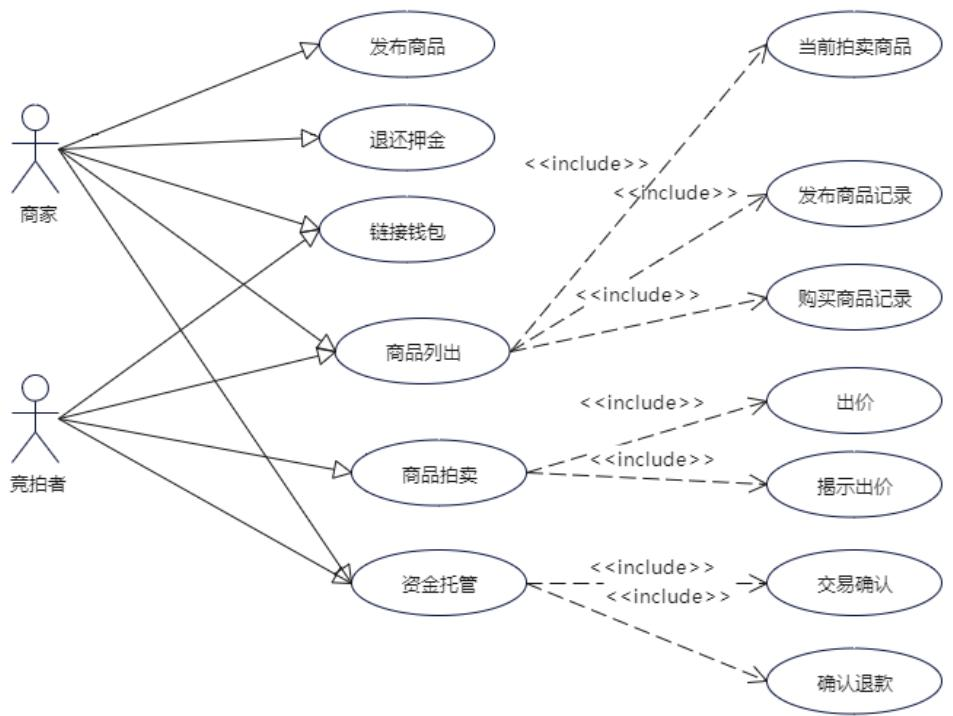
\includegraphics[keepaspectratio,alt={image}]{images/cb77b43189dad77af4d1695a333c6373756d70dda6e7dbb3007d0d3350257219.jpg}}

图 2-1 系统用例图

（1） 链接钱包：竞拍者及商家在使用平台任何交易功能时都必须链接 MetaMask

钱包到网站进行授权，授权后平台才能获取用户的钱包账户，从而进行签名的交易。

（2）
发布商品：商家可以在平台的``上传商品''页面，输入商品名称、选择商品分类、输入商品起拍价格、商品新旧条件、商品起拍时间、商品拍卖时长、点击选择上传的图片、输入商品描述，点击``立即添加商品''，进行上传商品。

（3） 退还押金：当商家发布的商品无人拍卖时，商家可申请退还押金。

（4）
商品列出：在平台首页将列出当前拍卖中的商品、用户购买的商品、用户发布的商品。列出的商品展示其名称、起拍价格、起拍时间、结束时间等。

（5）
商品拍卖：竞拍者可在商品详情页面对拍卖中的商品进行出价，出价时需输入理想出价、实际发送的
ETH、加密密码。出价阶段之后，可揭示自己的出价，揭示出价需输入参与出价时的理想出价与加密密码，查看是否中标。

（6）
资金托管：竞拍者在中标后，将调用合约把自己的付款转入托管合约，通过买卖双方的操作，再进行付款给买家，或者退款给自己。

\section{2.1.2
主要用例详细描述}\label{ux4e3bux8981ux7528ux4f8bux8be6ux7ec6ux63cfux8ff0}

在图2-1所示的用例中，对于此拍卖平台，涉及到的主要用例有商品发布、商品拍卖以及资金托管。

\section{（1）商品发布}\label{ux5546ux54c1ux53d1ux5e03}

表 2-1 商品发布需求表

{\def\LTcaptype{none} % do not increment counter
\begin{longtable}[]{@{}|l|l|@{}}
\toprule\noalign{}
\endhead
\bottomrule\noalign{}
\endlastfoot
\hline
用例、标识符 & 发布商品 \\
\hline
功能描述 & 用户将拍卖商品上传至系统 \\
\hline
使用人员 & 商户 \\
\hline
输入 & 商品名称、选择商品分类、商品起拍价格、商品新旧条件、商品起拍时
间、商品拍卖时长、商品图片、商品描述 \\
\hline
系统响应 &
判断输入合法，图片、描述是否为空，请求MetaMask钱包账户签名确认 \\
\hline
输出 &
若输入合法，用户确认签名并发送商品起拍价格10\%的ETH保证金，则上传商品成功，反之无法上传商品 \\
\hline
操作序列号 &
1、用户在上传商品页面输入商品相关信息；2、点击添加商品到区块链并使用钱包确认交易签名； \\
\hline
异常显示 & 1、``输入错误，请重新上传''；2、``交易失败，拒绝签名交易'' \\
\hline
\end{longtable}
}

用户在``上传商品''的前端页面输入商品名称、选择商品分类、输入商品起拍价格、商品新旧条件、商品起拍时间、商品拍卖时长、点击选择上传的图片、输入商品描述，点击``立即添加商品''后，前端先请求链接钱包账户，然后判断商品图片文件与商品简介是否为空，如果不为空，就将二者的数据添加到
IPFS，得到对应文件存储在 IPFS 的Hash
值，接下来将拍卖的起始时间转换为时间戳，与拍卖时长相加得到拍卖结束时间的时间戳，然后前端调用以太坊上的合约，将商品名称、分类、商品图片的
Hash、商品简介的Hash、起拍时间的时间戳、结束时间的时间戳、起拍价格、新旧条件、添加商品的用户的钱包账户等发送到以太坊上进行数据存储，并携带发送起拍价的
\(10 \%\) 的 ETH
到以太坊上的拍卖合约中作为上传本商品的保证金，以防止恶意上传商品的用户。当在MetaMask
钱包扩展中确认了这笔交易，消息发送成功后，则商品添加完成。

\section{（2）商品拍卖}\label{ux5546ux54c1ux62cdux5356}

表 2-2 用户出价需求表

{\def\LTcaptype{none} % do not increment counter
\begin{longtable}[]{@{}|l|l|@{}}
\toprule\noalign{}
\endhead
\bottomrule\noalign{}
\endlastfoot
\hline
用例、标识符 & 用户出价 \\
\hline
功能描述 & 用户对拍卖中的商品进行出价 \\
\hline
使用人员 & 竞拍者 \\
\hline
输入 & 理性出价、实际发送的 ETH、加密密码 \\
\hline
系统响应 & 判断输入合法性，理性出价＞起拍价格，实际发送的
ETH≥理想出价 \\
\hline
输出 & 若输入合法，用户确认签名并发送对应的 ETH
到拍卖合约，参与出价成功，反之提示参与出价失败 \\
\hline
操作序列号 & 1、用户在商品详情页面输入理性出价、实际发送的
ETH、加密密码；2、点击``确认拍卖''，并使用钱包确认交易签名； \\
\hline
异常显示 & ``交易失败，拒绝签名交易'' \\
\hline
\end{longtable}
}

表 2-3 用户揭示出价需求表

{\def\LTcaptype{none} % do not increment counter
\begin{longtable}[]{@{}|l|l|@{}}
\toprule\noalign{}
\endhead
\bottomrule\noalign{}
\endlastfoot
\hline
用例、标识符 & 用户揭示出价 \\
\hline
功能描述 & 用户对拍卖中的商品进行揭标 \\
\hline
使用人员 & 参与出价成功的竞拍者 \\
\hline
输入 & 理性出价、加密密码 \\
\hline
系统响应 & 判断理想价格和加密密码的加密 Hash
是否与出价时一致，判断是否为当前最高出价 \\
\hline
\end{longtable}
}

续表2-3 用户揭示出价需求表

{\def\LTcaptype{none} % do not increment counter
\begin{longtable}[]{@{}|l|l|@{}}
\toprule\noalign{}
\endhead
\bottomrule\noalign{}
\endlastfoot
\hline
用例、标识符 & 用户揭示出价 \\
\hline
输出 &
若输入的理想价格和加密密码匹配，用户确认签名，则揭标成功，否则揭标失败；理想出价若为当前最高出价，则保留理想出价，退还多余ETH到揭标账户，若不是，则退还全部出价。 \\
\hline
操作序列号 &
1、用户在商品详情页面输入理性出价、加密密码；2、点击``揭示出价''，并使用钱包确认交易签名； \\
\hline
异常显示 & ``交易失败，拒绝签名交易'' \\
\hline
\end{longtable}
}

商品拍卖流程图如图 2-2 所示。

\pandocbounded{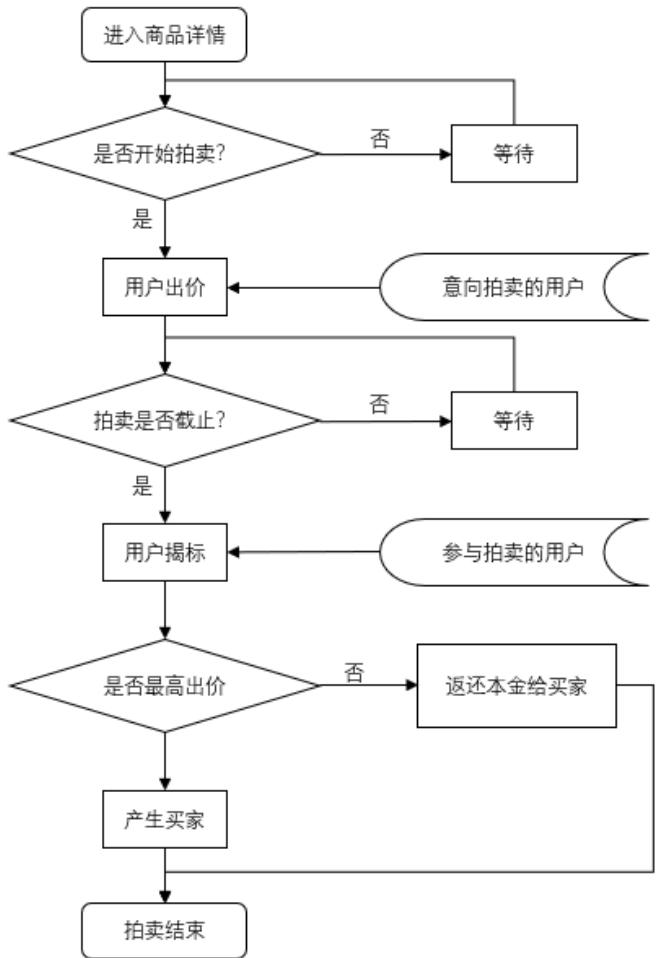
\includegraphics[keepaspectratio,alt={image}]{images/a774f4daaee8a242e862cf751051ddee630f8c858306c16cd2dce7133375a2e9.jpg}}

图 2-2 商品拍卖流程图

已授权网站连接到钱包账户的用户在首页中选择想要拍卖的商品，点击``商品详情''。平台前端会判断当前时间是否为拍卖时间，如果当前时间在拍卖开始时间到结束时间之间，则平台将显示商品图片，名称，分类，简介以及拍卖结束倒计时，竞拍者可以输入

理想出价、实际发送的
ETH、加密密码，然后点击``确认拍卖''，前端判断理想出价是否大于起拍价格、实际发送的
ETH 是否大于理想出价，二者都满足，则将理想出价与加密密码一起通过sha256
加密函数进行加密生成一个 Hash
值，然后调用以太坊的拍卖合约将商品对应的productId
和此加密Hash值发送到以太坊上进行数据存储，并且发送实际发送的ETH到拍卖合约，同时竞拍者在
MetaMask
钱包中签名确认交易，等到网络的其他节点确认完成后，即参与拍卖成功；如果当前时间在拍卖结束时间之后，则显示揭标输入框，用户可以输入参与竞拍时设置的理想价格和加密密码进行揭标。若不是最高出价者，则全额退款，若是最高出价者，则保留理想出价的资金部分，退回实际发送的ETH与理想出价之间多余对的差额。

\section{（3）资金托管}\label{ux8d44ux91d1ux6258ux7ba1}

当拍卖结束后，系统确定了卖家，买卖双方将进入资金托管合约，对交易资金进行处理。

\pandocbounded{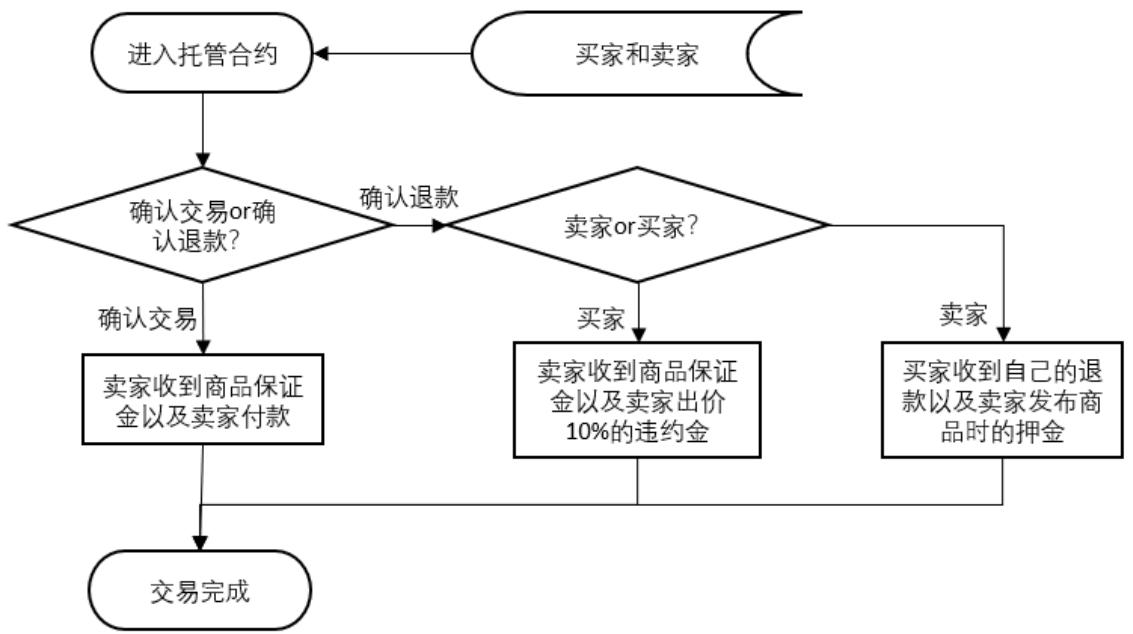
\includegraphics[keepaspectratio,alt={image}]{images/c187b2683c2d41ad605423a6cdadaf76018bcc83ddaa1d9533fcda8f1967e71f.jpg}}

图 2-3 资金托管流程图

其流程图如图2-3
所示，拍卖结束后，页面将展示最高出价者和买家的钱包地址以及成交价格。前端判断当前链接的钱包账户是否为卖家或最高出价者，最高出价者与卖家均可点击``进入托管合约''，通过钱包账户签名确认调用拍卖合约的敲定函数，拍卖合约会自动生成一个新的托管合约，并将卖家的保证金以及买家的出价资金转入该合约，进入托管合约后，买家与卖家可进行交易确认或退款操作。当买家与卖家都点击了``确认交易''之后，卖家可获得买家的付款以及添加商品时的保证金；当买卖双方其中一人

先点击``申请退款''后，则先点击的一方将被扣除一部分保证金给对方，买家违约退款，将扣除成交价
\(10 \%\) 的 ETH；卖家违约退款，将扣除上传商品时所付的所有 ETH。

\section{2.2 非功能需求}\label{ux975eux529fux80fdux9700ux6c42}

本系统是一个轻量级的区块链拍卖平台，作为一个去中心化的
Dapp，能够帮助撮合买卖双方进行更加安全、可信的商品拍卖交易，并提供友好的操作界面及展示效果。非功能需求包括以下几方面：

\section{（1）兼容性}\label{ux517cux5bb9ux6027}

该系统前端用Web 页面与用户交互，使用 Web3.js
与以太坊网络的智能合约进行交互。系统要拥有良好的兼容性，可以在
Windows、MacOS、Linux 等各种大主流操作系统上运行使用，同时兼容
Chrome、Firefox等。

\section{（2）继承性}\label{ux7ee7ux627fux6027}

该系统的建设和更新必须在保证不改变原有基础设计架构上进行，可以在保护正在进行的拍卖和交易的同时实现旧平台的更新和功能性升级。

\section{（3）易用性}\label{ux6613ux7528ux6027}

该系统的操作界面简单实用，页面布局合理，功能按钮描述简单明了，给用户提供可能出现的错误操作提示。用户可以很快速的掌握如何添加商品、拍卖出价、揭示出价、交易确认等系统的常规操作。

\section{（4）安全性}\label{ux5b89ux5168ux6027}

该系统的数据都是通过区块链加密传输，所有数据都存储在区块链上，保证隐私安全。合约代码都通过严格的审计，确保不出现任何合约漏洞，保证用户的资产安全。

\section{（5）稳定性}\label{ux7a33ux5b9aux6027}

该系统应该具有良好的容错能力，能够对系统可能出现的一些运行错误进行处理。保证系统可以稳定的运行。

\section{2.3 本章小结}\label{ux672cux7ae0ux5c0fux7ed3-1}

本章首先阐述了系统的功能性需求，使用系统用例图对系统所需的功能进行了分析，对涉及的主要功能用流程图以及相关描述确定了实现要求，并且提出了兼容性、继承性、易用性、安全性、稳定性五个方面的非功能性需求，保证系统更加完善。为后续的系统设计以及代码编写明确了方向和思路。

\section{第3章
区块链拍卖平台概要设计}\label{ux7b2c3ux7ae0-ux533aux5757ux94feux62cdux5356ux5e73ux53f0ux6982ux8981ux8bbeux8ba1}

\section{3.1 系统结构设计}\label{ux7cfbux7edfux7ed3ux6784ux8bbeux8ba1}

本系统基于 Truffle 框架开发的 Dapp，基于以太坊通过 Solidity
语言编写智能合约完成系统的后端逻辑，为系统前端提供合约函数接口，基于
IPFS（星际文件系统）实现图片、描述等大文件数据的分布式存储，基于 Vue
实现系统前端应用程序，基于 Web3完成前端代码与区块链以太坊以及 IPFS
的交互，使用 Node.js
作为系统运行前端应用程序的服务器。系统结构如图3-1所示：

\pandocbounded{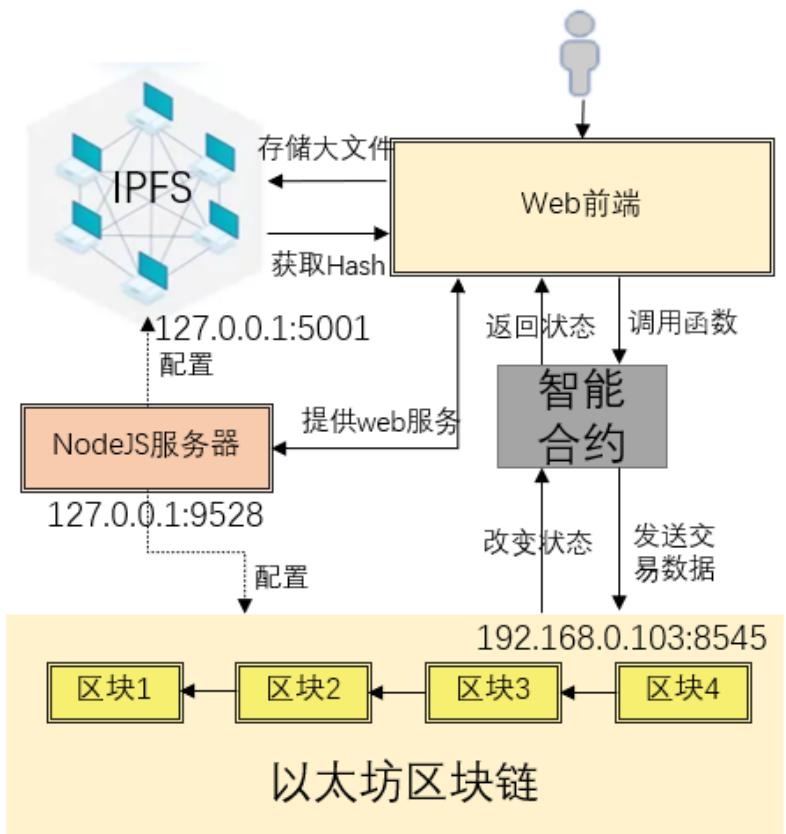
\includegraphics[keepaspectratio,alt={image}]{images/d25e10f2759fa3f17296cc811187a5cee624d80c5c1a30dbef9484c72d49928a.jpg}}

图 3-1 系统结构图

Web 前端：Html、Css 和 Javascript (Web3.js)，用户将通过 Web3.js
使前端应用程序与以太坊、IPFS 进行交互，前端应用程序就运行在 Nodejs
服务器上。

以太坊区块链：系统的核心部分，系统的智能合约就是部署在以太坊区块链上，系统中的所有商品信息、用户出价的
ETH也都是通过以太坊区块链进行分布式存储。

智能合约：智能合约主要实现系统的后端逻辑，为前端应用程序提供相对应的函数接口。通过
Web3.js 调用智能合约，在以太坊区块链上产生交易信息，实现系统的所有

功能。

Nodejs 服务器：Web 前端可以通过Nodejs 与以太坊区块链进行通信。

IPFS：当用户添加商品时，前端会将商品的图片和简介的文件数据上传到
IPFS，IPFS 会返回对应数据的 Hash 值{[}15{]}，并且将此 Hash
值存储到以太坊区块链中。

\section{3.2 系统功能设计}\label{ux7cfbux7edfux529fux80fdux8bbeux8ba1}

按照需求的用例分析，将系统功能模块分为链接钱包模块、商品添加模块、商品列出及搜索模块、商品拍卖模块、资金托管模块。其功能结构图如图3-2所示。

\pandocbounded{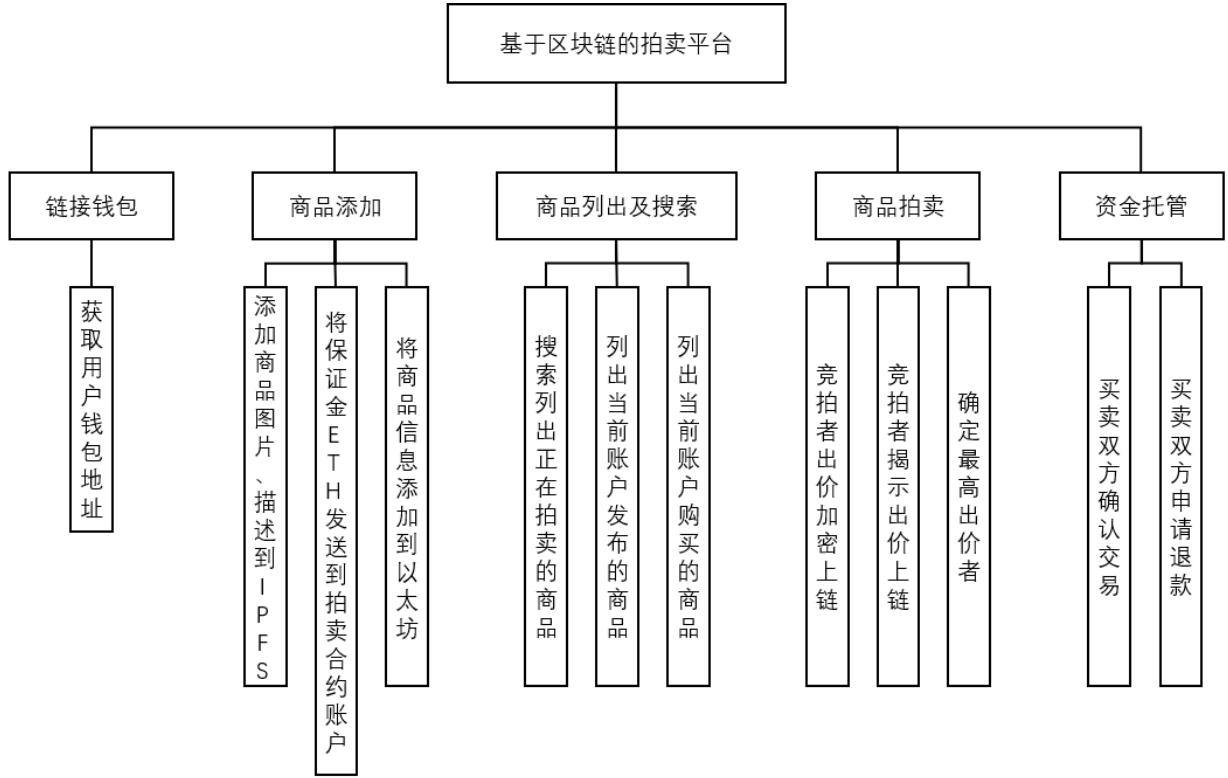
\includegraphics[keepaspectratio,alt={image}]{images/1ead5317947ff58615449d4208ab2428cbcb40873eb6894f26eade0248ba0e5d.jpg}}

图 3-2 功能结构图

\section{3.2.1 链接钱包模块}\label{ux94feux63a5ux94b1ux5305ux6a21ux5757}

此模块主要是获取用户的 MetaMask 钱包账户作为用户进行登录及使用平台。

用户进入平台首页，点击``链接钱包''，前端会检查用户是否安装 MetaMask
钱包插件，如果已经安装了，就会弹出 MetaMask
钱包扩展窗口，提示输入钱包密码，然后授权网站链接当前钱包的私钥账户，钱包链接成功；如果没有安装
MetaMask 钱包插件，则提示你没有安装，会在控制台显示安装 MetaMask
钱包插件的网址。用户将钱包授权链接到系统网站之后，才能够进行后续的商品添加、商品拍卖等功能。

\section{3.2.2
商品添加功能模块}\label{ux5546ux54c1ux6dfbux52a0ux529fux80fdux6a21ux5757}

此模块主要负责通过调用以太坊上的智能合约函数将用户输入的商品信息传输到以太坊上进行分布式的存储。

用户在``上传商品''的前端页面输入商品名称、选择商品分类、输入商品起拍价格、商品新旧条件、商品起拍时间、商品拍卖时长、点击选择上传的图片、输入商品描述，点击``立即添加商品''后，前端先请求链接钱包账户，然后判断商品图片文件与商品简介是否为空，如果不为空，就将二者的数据添加到
IPFS，得到对应文件存储在 IPFS 的Hash
值，接下来将拍卖的起始时间转换为时间戳，与拍卖时长相加得到拍卖结束时间的时间戳，然后前端调用以太坊上的合约函数，将商品名称、分类、商品图片的
Hash、商品简介的Hash、起拍时间的时间戳、结束时间的时间戳、起拍价格、新旧条件、添加商品的用户的钱包账户等发送到以太坊上，进行数据存储，并携带发送起拍价的
\(10 \%\) 的ETH
到以太坊上的拍卖合约中作为上传本商品的保证金，以防止恶意上传商品的用户。当在MetaMask
钱包扩展中确认了这笔交易，消息发送成功后，则商品添加完成。

\section{3.2.3
商品列出及搜索模块}\label{ux5546ux54c1ux5217ux51faux53caux641cux7d22ux6a21ux5757}

此模块主要是将已经添加到以太坊区块链上的商品进行展示，并提供通过名称搜索商品的功能。

商品展示顺序将按照上传商品的时间顺序进行，因为每上传一件商品在以太坊区块链上，那么那件商品都有自己独特的
ID，使用 Web3.js 可以通过遍历产品 ID
得到每件商品的商品信息并展示到前端页面中；当用户在搜索框输入商品名称对商品进行搜索时，只是增加了对于商品名称的值是否相等的判断，然后再展示到前端页面中。

除了展示正在拍卖的商品，还将展示该用户发布和购买商品的记录。

\section{3.2.4 商品拍卖模块}\label{ux5546ux54c1ux62cdux5356ux6a21ux5757}

此模块主要是完成商品拍卖出价到确定买家的过程的操作逻辑。商品的状态随着时间以及用户操作的改变而改变。商品拍卖状态图描述如图
3-3所示：

\pandocbounded{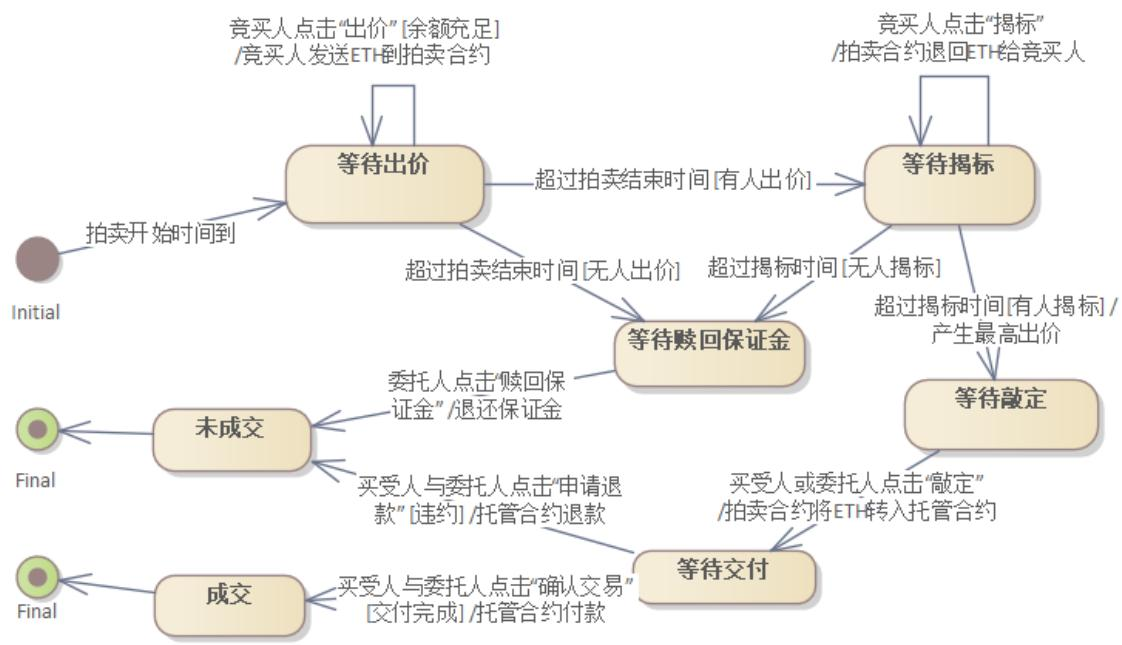
\includegraphics[keepaspectratio,alt={image}]{images/f899f9ad01eecaa8d9c45411b2e7481eb6689cab67c8530157924b9963a13b47.jpg}}

图 3-3 拍卖状态图

根据商品的状态不同判断商品拍卖的阶段，可分为 3个阶段：

第一阶段为出价阶段，竞拍者对商品进行出价，并且设置一个迷惑其他竞拍者的出价，因为任何人的出价都会被记录在以太坊的交易中，并且任何人都可以查看，所以针对本系统的密封拍卖方式，竞拍者需要设置一个迷惑出价（实际发送到拍卖合约的
ETH），并且设置一个密码来对理想出价进行加密，防止他人利用区块链的透明性知道竞争对手的出价而使密封拍卖失去公平性。

第二阶段为揭示出价阶段，揭示出价阶段被设置成
2小时，智能合约将自动锁定在这两小时之内对自己之前的出价进行揭示的账户中找到最高出价者，并将第二高出价设置为成交价。除了最高出价者以外的账户将在揭标时收到拍卖合约的资金退还。

第三个阶段为超时揭示出价者资金退回阶段，拍卖截止两小时之后揭示出价的竞拍者的竞拍无效，揭示出价时合约将退回该账户发送到拍卖合约的资金。

当商品无人拍卖时，商家可申请赎回上传商品时发送的ETH保证金。

\section{3.2.5 资金托管模块}\label{ux8d44ux91d1ux6258ux7ba1ux6a21ux5757}

此模块主要为商品的买卖双方提供资金托管服务。活动图如图3-4所示：

\pandocbounded{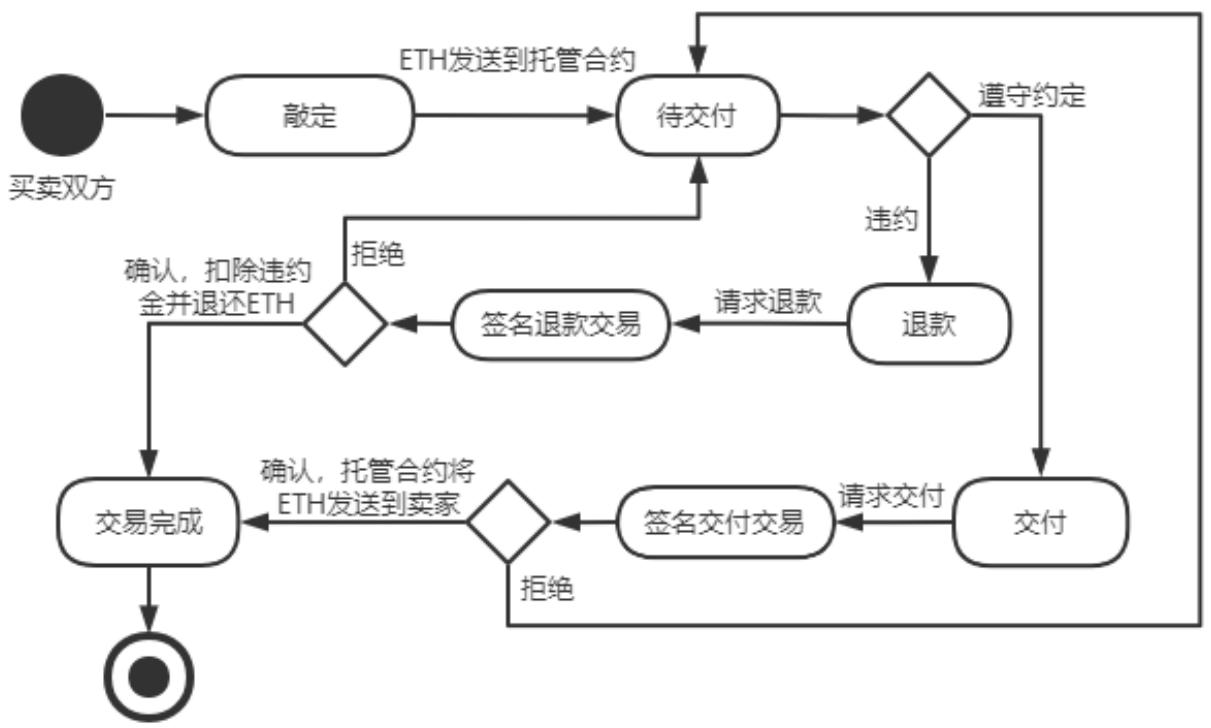
\includegraphics[keepaspectratio,alt={image}]{images/2e16dea9da807b4fb7192583b243f32ea2160df88851f1496f2780f0256945c8.jpg}}

图 3-4 资金托管活动图

当一件商品确定了最高出价者即买家之后，该买家对于该商品的成交价以及该商品的卖家的保证金，将发送到资金托管合约进行暂时的保管。当双方对于该商品对拍卖结果达成一致之后，合约将把相对应的资金发送到买家或卖家钱包账户中。

\section{3.3 本章小结}\label{ux672cux7ae0ux5c0fux7ed3-2}

本章根据需求首先确定了系统采用的整体架构，然后确定了五个功能模块并对其主要功能使用活动图进行了详细的描述，为后续系统的前后端各个功能的实现提供了更近进一步的帮助。

\section{第4章
区块链拍卖平台详细设计与实现}\label{ux7b2c4ux7ae0-ux533aux5757ux94feux62cdux5356ux5e73ux53f0ux8be6ux7ec6ux8bbeux8ba1ux4e0eux5b9eux73b0}

\section{4.1 智能合约}\label{ux667aux80fdux5408ux7ea6}

本系统使用 Solidity
语言作为智能合约的编程语言，可部署在以太坊公链上使用。区块链类型可分为公有链、联盟链、私有链。公有链即全球所有人都可以访问的区块链，并且谁都可以发送交易，合法的交易都可以被保存到区块链中，每个人都可以参与到一致性协商都过程中，一致性协商过程决定了哪个区块将会被保存到链上。因此公有链是完全去中心化的；联盟链是指一致性协商的过程是由一些预先选择好的节点控制的区块链，链上数据的查询权限能够公开，也能对某个成员节点进行限制，也能混合管理。因此联盟链是部分去中心化的；私有链是一条完全由个体掌握的区块链，只有一个中心化的组织拥有该区块链区块的写权限。可以由该组织自定义公开的读权限。所以私有链是一个中心化的区块链。

为了降低成本，通过 truffle 将智能合约部署在 ganache
搭建的以太坊测试链上。智能合约的设计主要将其分为 EcommerceStore
合约、Escrow
合约。其中，EcommerceStore合约主要是用于存储商品信息以及实现商品拍卖过程中的各个功能，将每个
Product 结构体使用 mapping 进行记录。Escrow
合约主要用于敲定后对买卖双方的资产进行管理。

对于智能合约代码的处理需要分三个步骤：编译合约、部署合约、调用合约。

\section{4.1.1 编译合约}\label{ux7f16ux8bd1ux5408ux7ea6}

在 truffle 框架下，只需要在命令行输入 truffle compile 即可编译生成合约的
json 文件，并存放在migrations 文件夹下。

\pandocbounded{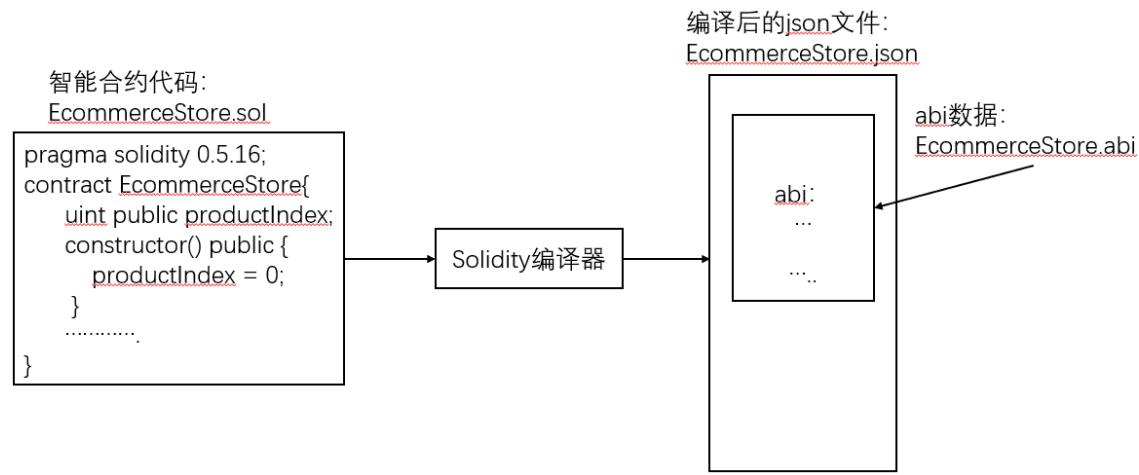
\includegraphics[keepaspectratio,alt={image}]{images/5eaeca7542f5eb4c5d98a7370187eb3c3a999ad98fa53e2e6a4172225046893a.jpg}}

图 4-1 智能合约编译过程

如图 4-1 所示。拍卖合约源代码 EcommerceStore.sol 在经过 Solidity
编译器编译后，生成 EcommerceStore.json 文件。

\section{4.1.2 部署合约}\label{ux90e8ux7f72ux5408ux7ea6}

在 truffle 框架下，命令行输入 truffle migrate --network
ganacheNet，即可在 ganache创建的以太坊区块链上部署 migrations
文件价下的合约文件。

\pandocbounded{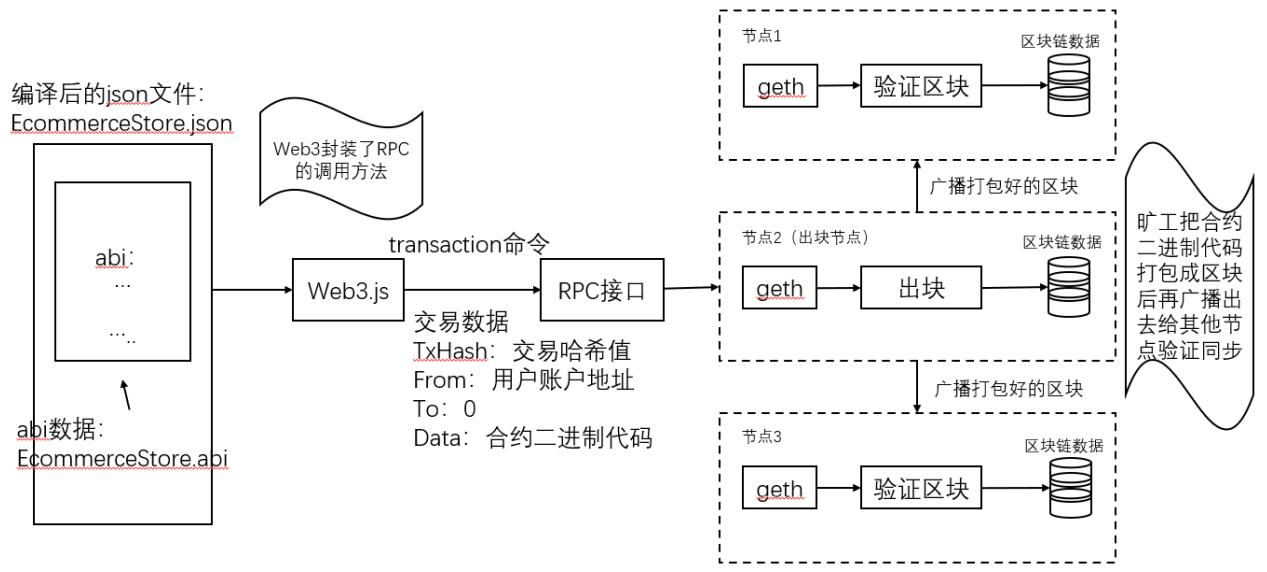
\includegraphics[keepaspectratio,alt={image}]{images/cb46f3305d43b00b846b2f5e410717f1ca4a55b0847402c5caecce3655889d48.jpg}}

图 4-2 智能合约部署过程

如图 4-2 所示，合约的部署跟发送一笔交易是一样的操作，调用 transaction
函数，from 为用户账户地址，to 为 0，data 为合约的 EVM
操作码。在矿工打包合约二进制代码后会生成智能合约地址。智能合约地址的生成是由合约发布者的账号和发送的交易数作为随机数输入，通过
Kecca-256加密算法创建的一个合约账户。换句话说，合约地址以及合约代码会对应的保存在区块链数据库。调用者只需要有合约地址和
abi 文件就可以调用合约的代码。

\section{4.1.3 调用合约}\label{ux8c03ux7528ux5408ux7ea6}

在前端的js文件中用require(`web3')来引入当前路径下安装的web3，创建一个Web3对象，然后再使用
web3.setProvider 连接到以太坊节点，引入合约的 json 文件，json
文件中包含合约abi，然后定义合约完成，即可调用其函数。

\pandocbounded{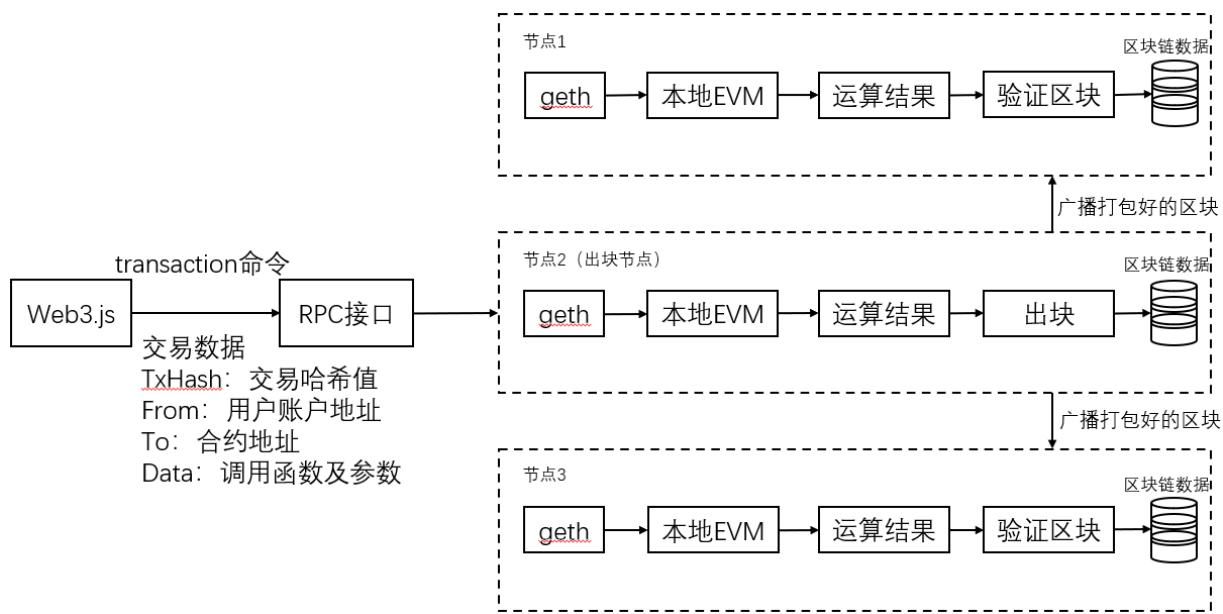
\includegraphics[keepaspectratio,alt={image}]{images/09ef59c244fa40c477eba0aaefd37e084d911b3a99243cae520c4b1ff42179bc.jpg}}

图 4-3 智能合约调用过程

调用合约需要合约的地址和合约的方法，如图
4-3所示，智能合约是部署在区块链的代码，区块链本身不能执行代码，代码的执行是在本地的
EVM
中，实际上，部署在区块链上代码是能够在本地产生原生智能合约代码，可以理解区块链为一个数据库，而客户端从数据库中读取了存储的运行代码，并在本地运行后，将结果写入到了区块链这个数据库中。

\section{4.1.4
合约函数功能及参数说明}\label{ux5408ux7ea6ux51fdux6570ux529fux80fdux53caux53c2ux6570ux8bf4ux660e}

EcommerceStore 拍卖合约中函数功能以及参数说明如表 4-1 所示。

表 4-1 EcommerceStore 拍卖合约函数功能及参数表

{\def\LTcaptype{none} % do not increment counter
\begin{longtable}[]{@{}|l|l|l|l|@{}}
\toprule\noalign{}
\endhead
\bottomrule\noalign{}
\endlastfoot
\hline
函数名 & 功能 & 参数 & 返回值 \\
\hline
numberOfItems() & 获取当前商品数量 & 无 & uint productIndex \\
\hline
getAccountOfId() & 获取产品上传者地址 & uint\_productId & address \\
\hline
bid() & 用户对商品出价 & uint\_productIdbytes32\_bytesHash & 无 \\
\hline
totalBids() & 获取当前商品竞拍人数 & uint\_productId & uint
product.totalBids \\
\hline
\end{longtable}
}

续表 4-1 EcommerceStore 拍卖合约函数功能及参数表

{\def\LTcaptype{none} % do not increment counter
\begin{longtable}[]{@{}llll@{}}
\toprule\noalign{}
\endhead
\bottomrule\noalign{}
\endlastfoot
函数名 & 功能 & 参数 & 返回值 \\
\multirow{11}{*}{addProductToStore()} &
\multirow{11}{*}{添加商品信息到区块链} & string memory\_name & \\
& & string memory & \\
& & \_category & \\
& & string memory & \\
& & \_imageLink & \\
& & string memory & 无 \\
& & descLink & \\
& & uint\_auctionStartTime & \\
& & uint\_auctionEndTime & \\
& & uint\_startPrice & \\
& & uint\_productCondition & \\
\multirow{11}{*}{getProductByld()} & \multirow{11}{*}{获取商品信息} &
\multirow{11}{*}{uint\_productId} & uint product.id \\
& & & string memory product.name \\
& & & string memory product(category) \\
& & & string memory product(imageLink \\
& & & string memory product.auctionStartTime \\
& & & product.auctionEndTime \\
& & & uint product.auctionStartTime \\
& & & uint product.auctionEndTime \\
& & & uint product.startPrice \\
& & & uint product.status \\
& & & uint product.statusCondition \\
\multirow{3}{*}{revealBid()} & \multirow{3}{*}{用户揭示商品出价} &
uint\_productId & \\
& & uint\_AdealPrice & 无 \\
& & string memory\_secret & \\
\end{longtable}
}

续表 4-1 EcommerceStore 拍卖合约函数功能及参数表

{\def\LTcaptype{none} % do not increment counter
\begin{longtable}[]{@{}|l|l|l|l|@{}}
\toprule\noalign{}
\endhead
\bottomrule\noalign{}
\endlastfoot
\hline
函数名 & 功能 & 参数 & 返回值 \\
\hline
getHighestBidInfo() & 获取最高出价者地址、最高出价、第二高出价、竞标人数
& uint\_productId & address product.highestBidderuint
product.highestBiduint product(secondHighestBiduint product.totalBids \\
\hline
finalizeAuction() & 敲定，将买卖双方的交易资金存入托管合约 &
uint\_productId & 无 \\
\hline
getEscrowInfo() & 获取托管合约信息 & uint\_productId & address
buyeraddress sellerbool fundsDisburseduint releaseCountuint
refundCountuint buyerAmountuint sellerDesposittuint createTime \\
\hline
releaseAmountToSeller() & 向卖家付款 & uint\_productId & 无 \\
\hline
refundAmountToBuyer() & 向买家退款 & uint\_productId & 无 \\
\hline
\end{longtable}
}

\section{4.2
系统功能模块设计与实现}\label{ux7cfbux7edfux529fux80fdux6a21ux5757ux8bbeux8ba1ux4e0eux5b9eux73b0}

\section{4.2.1
链接钱包模块}\label{ux94feux63a5ux94b1ux5305ux6a21ux5757-1}

\section{（1）实现过程}\label{ux5b9eux73b0ux8fc7ux7a0b}

该模块中，前端首先检测 MetaMask 插件是否安装，这里引入了 \(@\)
metamask/detect-provider 模块，通过该模块的
detectEthereumProvider()函数对 provider 进行赋值，然后判断 provider
是否被定义，如果 provider 为 undefined，则表示为安装 MetaMask 插件；如果
provider 不为 undefind，则表示已经安装了 MetaMask 插件。接下来就是
MetaMask 授

权，通过调用 eth\_requestAccounts 方法进行 MetaMask 授权，用户若在
MetaMask
钱包扩展中确认授权，则网站链接钱包成功；拒绝授权，则网站链接钱包失败，用户将无法使用系统。

\section{（2）关键代码}\label{ux5173ux952eux4ee3ux7801}

该模块的关键代码如代码 4-1所示。

代码 4-1 链接钱包模块关键代码

\begin{Shaded}
\begin{Highlighting}[]
\ImportTok{import}\NormalTok{ detectEthereumProvider }\ImportTok{from} \StringTok{\textquotesingle{}@metamask/detect{-}provider\textquotesingle{}}  
\CommentTok{//检查是否安装MetaMask插件  }
\KeywordTok{var}\NormalTok{ provider }\OperatorTok{=} \ControlFlowTok{await} \FunctionTok{detectEthereumProvider}\NormalTok{()}\OperatorTok{;}  
\ControlFlowTok{if}\NormalTok{ (provider) \{  }
    \CommentTok{// provider == window.etherum  }
\NormalTok{\} }\ControlFlowTok{else}\NormalTok{ \{  }
    \KeywordTok{this}\NormalTok{ $}\OperatorTok{.}\FunctionTok{notify}\NormalTok{(\{}
        \DataTypeTok{title}\OperatorTok{:} \StringTok{"提示"}\OperatorTok{,}
        \DataTypeTok{message}\OperatorTok{:} \StringTok{"您未安装MetaMask插件"}
\NormalTok{    \})}\OperatorTok{;}  
\NormalTok{\}  }
\CommentTok{//MetaMask授权  }
\KeywordTok{const}\NormalTok{ a }\OperatorTok{=} \ControlFlowTok{await}\NormalTok{ etherum}\OperatorTok{.}\FunctionTok{request}\NormalTok{(\{ }\DataTypeTok{method}\OperatorTok{:} \StringTok{"eth\_requestAccounts"}\NormalTok{\})；}
\end{Highlighting}
\end{Shaded}

\section{（3）界面展示}\label{ux754cux9762ux5c55ux793a}

该模块的前端页面如图所示，点击链接钱包的按钮，MetaMask
扩展程序将弹出使用钱包账户链接到网站的提示，如图 4-4 所示，点击 Connect
按钮，即可将钱包账户授权到网站，如图4-5所示，前端页面将显示该账户的地址信息，从而成为系统用户。

\pandocbounded{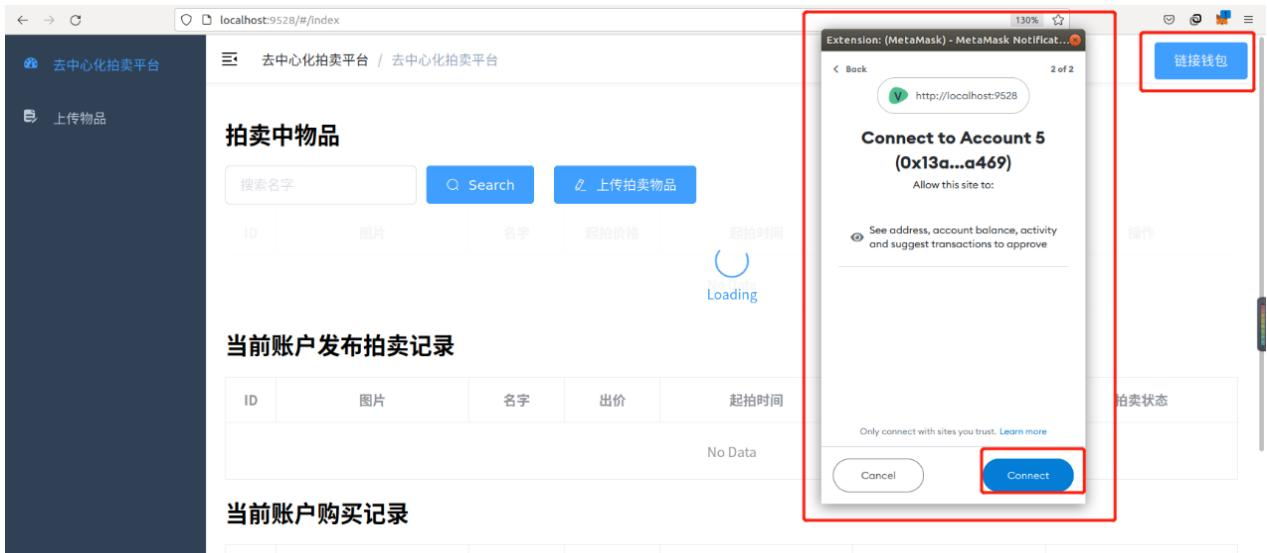
\includegraphics[keepaspectratio,alt={image}]{images/6bc4180b0ccb0bf15bad358012e91259677bcc325b967adc678eff4db30251c5.jpg}}

图 4-4 链接钱包请求截图

\pandocbounded{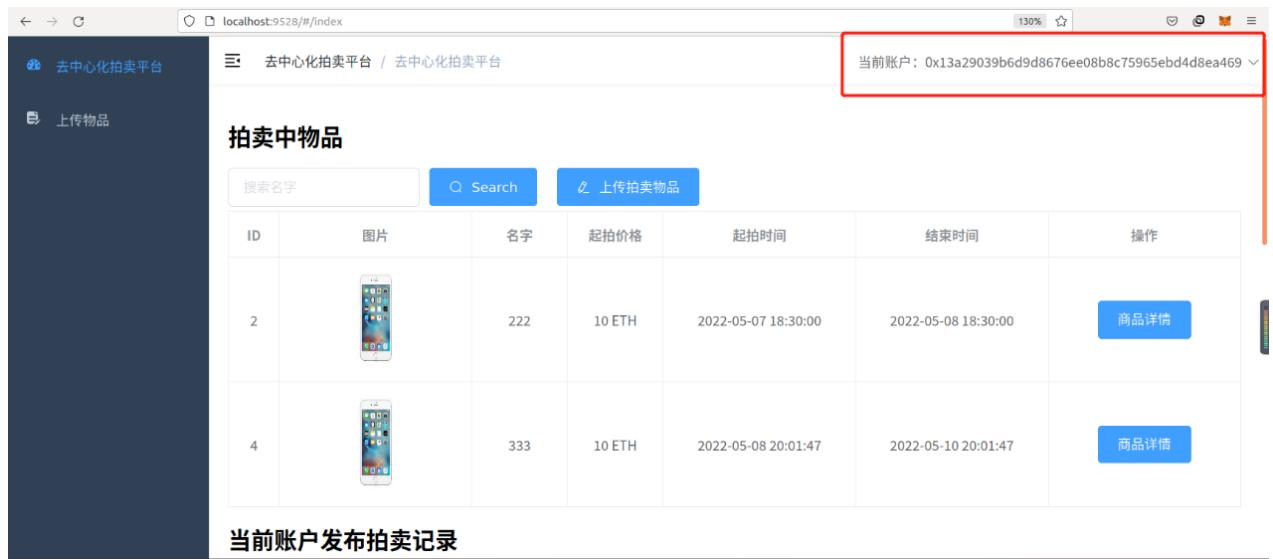
\includegraphics[keepaspectratio,alt={image}]{images/52395d2c367ea9cbbc7bbab532703b4df2eb3386b514d48c8437380edac8a381.jpg}}

图 4-5 链接钱包后前端展示账户

\section{4.2.2 商品添加模块}\label{ux5546ux54c1ux6dfbux52a0ux6a21ux5757}

\section{（1）实现过程该模块}\label{ux5b9eux73b0ux8fc7ux7a0bux8be5ux6a21ux5757}

在用户输入商品的所有信息后，点击``立即添加商品''，前端首先判断图片文件以及简介是否为空，如果为空就在控制台提示，重新点击添加；如果不为空，则将二者的副本数据添加到
IPFS 中，返回得到该数据在 IPFS 的存储 Hash
值，前端又通过起拍时间与拍卖时长计算出拍卖结束时间，将拍卖开始时间与拍卖结束时间转换为时间戳的形式。最后再调用合约函数将商家保证金发送到拍卖合约、商品信息添加到以太坊区块链中。

\section{（2）关键代码}\label{ux5173ux952eux4ee3ux7801-1}

该模块的合约关键代码如代码 4-2所示。

代码 4-2 商品添加模块合约关键代码

\begin{Shaded}
\begin{Highlighting}[]
\NormalTok{//添加商品到区块链  }
\NormalTok{function addProductToStore(string memory\_name, string memory\_category, string memory\_imageLink, string memory\_descLink, uint\_startTime, uint\_endTime, uint\_startPrice, uint condition) payable public \{  }
\NormalTok{    require(\_startTime \textless{} \_endTime);  }
\NormalTok{    uint\_deposit = \_startPrice.div(10);  }
\NormalTok{    require(msg.value \textgreater{}= \_deposit);  }
\NormalTok{    productIndex = productIndex.add(1);  }
\NormalTok{    Product memory product = Product(\{  }
\NormalTok{        id: productIndex, //商品ID  }
\NormalTok{        name:\_name, //商品名称  }
\NormalTok{        category:\_category, //商品分类}
\end{Highlighting}
\end{Shaded}

\begin{Shaded}
\begin{Highlighting}[]
\NormalTok{imageLink}\OperatorTok{:}\NormalTok{\_imageLink}\OperatorTok{,} \CommentTok{//商品图片Hash  }
\NormalTok{descLink}\OperatorTok{:}\NormalTok{\_descLink}\OperatorTok{,} \CommentTok{//商品描述Hash  }
\NormalTok{startPrice}\OperatorTok{:}\NormalTok{\_startPrice}\OperatorTok{,} \CommentTok{//商品起拍价格  }
\NormalTok{auctionStartTime}\OperatorTok{:}\NormalTok{\_startTime}\OperatorTok{,} \CommentTok{//拍卖开始时间  }
\NormalTok{auctionEndTime}\OperatorTok{:}\NormalTok{\_endTime}\OperatorTok{,} \CommentTok{//拍卖结束时间  }
\NormalTok{status}\OperatorTok{:}\NormalTok{ ProductStatus}\OperatorTok{.}\AttributeTok{Open}\OperatorTok{,} \CommentTok{//商品状态  }
\NormalTok{condition}\OperatorTok{:} \FunctionTok{ProductCondition}\NormalTok{(condition)}\OperatorTok{,} \CommentTok{//商品条件  }
\NormalTok{highestBid}\OperatorTok{:}\DecValTok{0}\OperatorTok{,} \CommentTok{//最高出价  }
\NormalTok{highestBidder}\OperatorTok{:}\FunctionTok{address}\NormalTok{(}\DecValTok{0}\NormalTok{)}\OperatorTok{,} \CommentTok{//最高出价者  }
\NormalTok{secondHighestBid}\OperatorTok{:}\DecValTok{0}\OperatorTok{,} \CommentTok{//第二高出价  }
\NormalTok{totalBids}\OperatorTok{:}\DecValTok{0}\OperatorTok{,} \CommentTok{//商品出价人数  }
\NormalTok{deposit}\OperatorTok{:}\NormalTok{msg}\OperatorTok{.}\AttributeTok{value} \CommentTok{//商品押金  }
\NormalTok{\})}\OperatorTok{;}  
\NormalTok{emit新产品}\OperatorTok{.}\AttributeTok{productIndex}\OperatorTok{,}\NormalTok{\_name}\OperatorTok{,}\NormalTok{\_category}\OperatorTok{,}\NormalTok{\_imageLink}\OperatorTok{,}\NormalTok{\_descLink}\OperatorTok{,}\NormalTok{\_startTime}\OperatorTok{,}\NormalTok{\_endtime}\OperatorTok{,}\NormalTok{\_startPrice}\OperatorTok{,}\NormalTok{\_condition}\OperatorTok{,}\NormalTok{ msg sender)}\OperatorTok{;}  
\NormalTok{stores[msgsender][productIndex] }\OperatorTok{=}\NormalTok{ product}\OperatorTok{;}  
\NormalTok{productIdToOwnerazesProductIndex }\OperatorTok{=}\NormalTok{ msgsender}\OperatorTok{;}
\end{Highlighting}
\end{Shaded}

\section{（3）界面展示}\label{ux754cux9762ux5c55ux793a-1}

该模块的前端页面展示如图
4-6所示，用户商品信息录入网页，点击``立即添加商品''，然后在MetaMask
扩展程序点击confirm
进行签名确认交易，交易确认完成即可添加成功，最后是首页对上传商品的展示，如图
4-7所示。

\pandocbounded{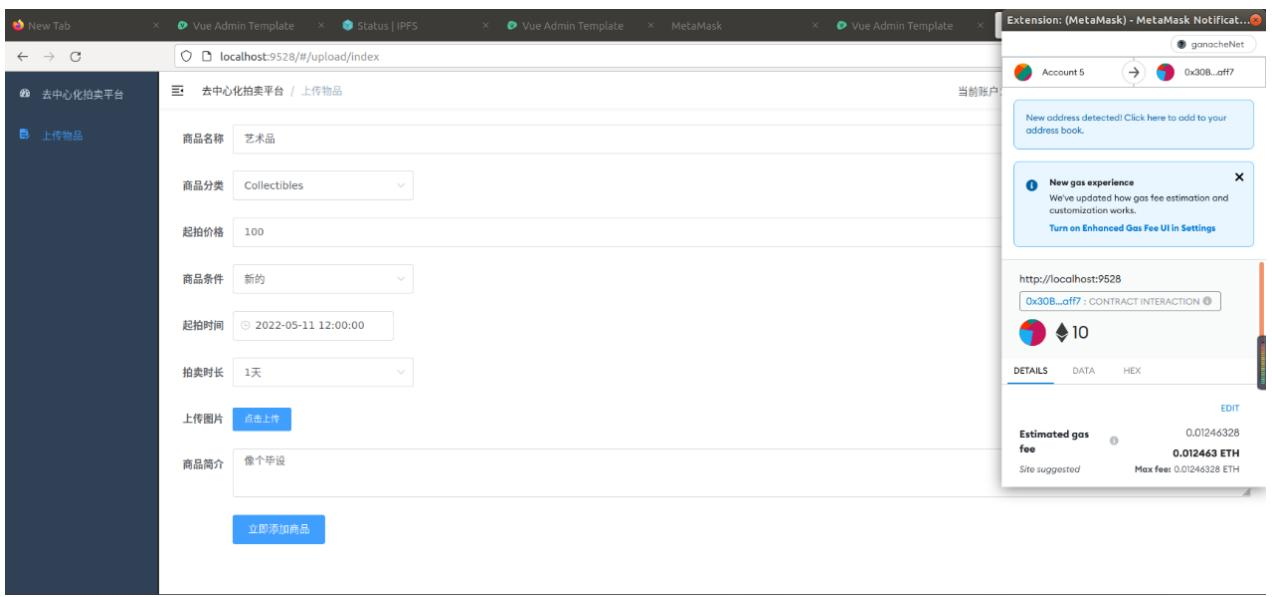
\includegraphics[keepaspectratio,alt={image}]{images/f39b024839f5a43d88388014b6edf752b4219be4412f18a32076c9099f0d71a8.jpg}}

图 4-6 商品添加模块钱包确认截图

\pandocbounded{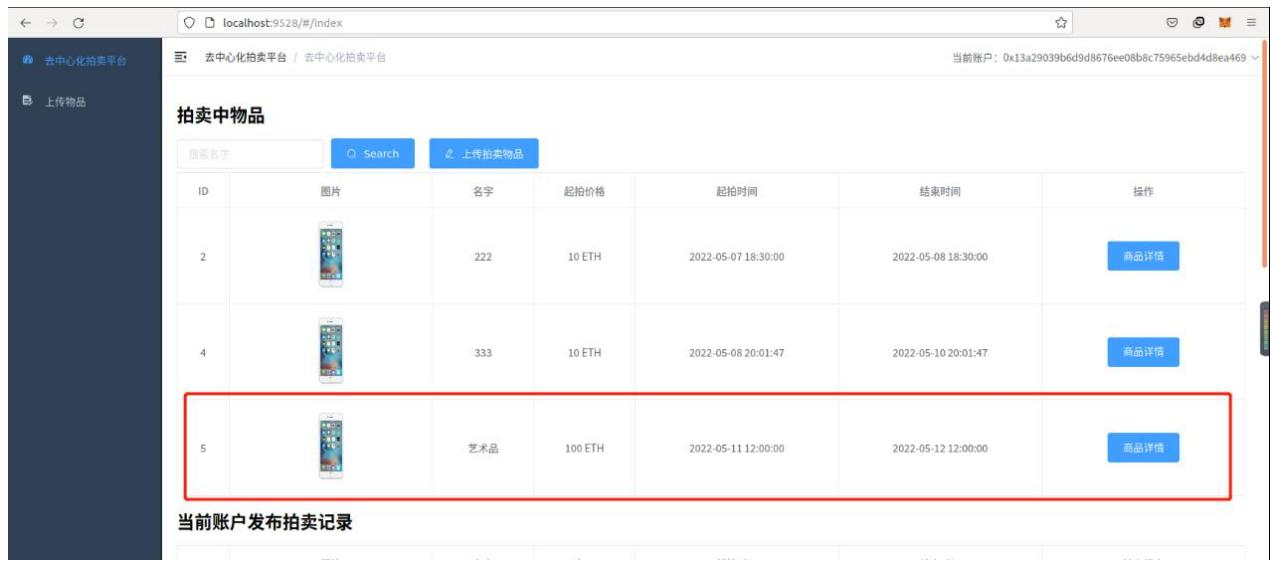
\includegraphics[keepaspectratio,alt={image}]{images/376aa85cb7557ec628d3ce38e1c1461569003c65b7f7ec76ba8c65b7f078d1f7.jpg}}

图 4-7 商品添加模块成功添加商品首页截图

\section{4.2.3
商品列出及搜索模块}\label{ux5546ux54c1ux5217ux51faux53caux641cux7d22ux6a21ux5757-1}

\section{（1）实现过程}\label{ux5b9eux73b0ux8fc7ux7a0b-1}

该模块主要列出即将开始拍卖或拍卖中商品、当前账户发布拍卖记录、当前账户购买记录，并且增加了按商品名称搜索的功能。前端代码中主要就是遍历合约中的每一个商品信息，将图片以及简介的
Hash 在IPFS
网络中查询，找到相应的副本文件，展示到页面，然后通过商品发布者、商品最高出价者、商品的状态使用过滤器对商品进行筛选，分别展示在对应的页面下方。

\section{（2）关键代码}\label{ux5173ux952eux4ee3ux7801-2}

该模块的合约关键代码如代码 4-3 所示。

代码 4-3 商品列出及搜索模块合约关键代码

\begin{Shaded}
\begin{Highlighting}[]
\NormalTok{//通过商品编号获取商品信息  }
\NormalTok{function getProductByld( uint \_productId) view public returns uint, string memory, string memory, string memory, string memory, uint, uint, uint, uint, address, uint) \{  }
\NormalTok{    address owner = productIdToOwner\_[productId];  }
\NormalTok{    Product memory product = stores[owner][\_productId];  }
\NormalTok{    return (product.id, product.name, product category, product(imageLink, product DESCLink, product.auctionStartTime, product.auctionEndTime, product.startPrice, uint( product.status), product.highestBidder, product.highestBid));  }
\NormalTok{\}}
\end{Highlighting}
\end{Shaded}

\section{（3）界面展示}\label{ux754cux9762ux5c55ux793a-2}

该模块的页面展示如图 4-8 所示。

\pandocbounded{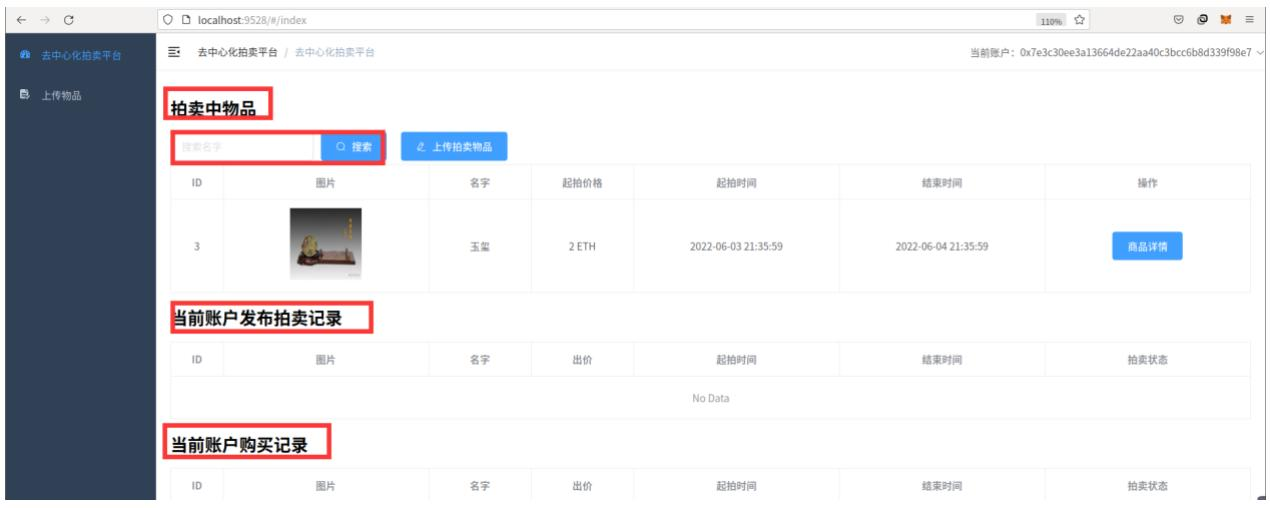
\includegraphics[keepaspectratio,alt={image}]{images/d035d4e23a01924f3f9b115fdcb90f2d0d5afc37129a1e44369d30af0f6cd629.jpg}}

图 4-8 商品列出及搜索模块界面

\section{4.2.4
商品拍卖模块}\label{ux5546ux54c1ux62cdux5356ux6a21ux5757-1}

该模块对用户的出价以及用户的揭示出价进行了处理，确定最高出价者即买家。买家才有资格进行敲定。拍卖实现流程图如图
4-9所示。

\pandocbounded{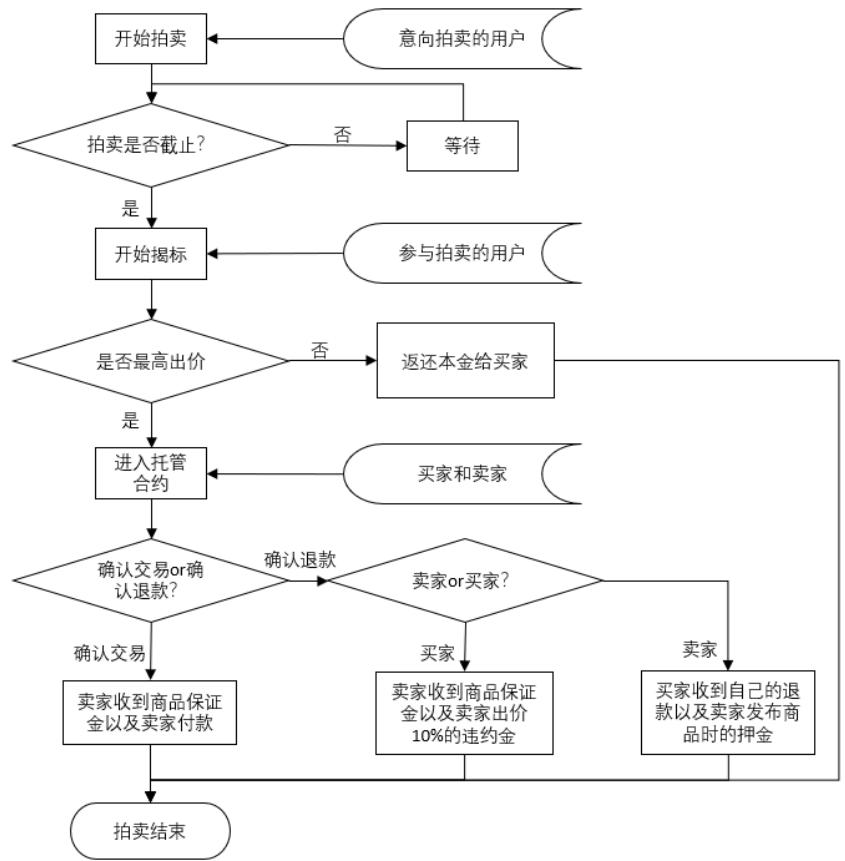
\includegraphics[keepaspectratio,alt={image}]{images/6664c0a16f865a85dea19256a110acb04962134e1fb19878c23b976b7c9ba2ab.jpg}}

图 4-9 商品拍卖流程图

\section{（1）实现过程}\label{ux5b9eux73b0ux8fc7ux7a0b-2}

首先是通过调用 EcommerceStore 合约的
getProductById()函数获取当前商品的商品信息，接下来就是根据时间以及用户身份来展示不同的前端页面提示。如果当前时间在拍卖开始时间之前，则商品详情页将显示``该商品还未开始拍卖，请等待''；如果当前时间在拍卖开始时间之后，拍卖结束时间之前，则商品详情页将对竞拍者显示出价页面，如图
4-10 所示，点击``出价''即调用
bid()函数；对卖家显示``你的商品正在竞拍中，请等待''；如果当前时间在拍卖结束之后
2 小时内，则商品详情页将对竞拍者显示揭示出价页面，点击``揭标''即调用
revealBid()；对未参与竞拍的用户显示``你未参与拍卖，拍卖已结束''，对卖家显示``你的商品正在揭标中，请等待''；如果当前时间超过了拍卖结束之后2小时，则商品详情页将向所有用户公布卖家与买家以及成交价。如果有用户参与了出价，但未在规定时间揭标，则将为该用户开通赎回资产的功能。

\section{（2）关键代码}\label{ux5173ux952eux4ee3ux7801-3}

该模块的合约关键代码如代码 4-4 所示。

代码 4-4 商品拍卖模块关键代码

\begin{Shaded}
\begin{Highlighting}[]
\NormalTok{//参与出价  }
\NormalTok{function bid( uint \_productId, bytes32\_bytesHash) payable public \{  }
\NormalTok{Product storage product = stores[产品质量ToOwner[\_productId]][\_productId];  }
\NormalTok{require(now \textgreater{}= product.auctionStartTime);  }
\NormalTok{require(now \textless{}= product.auctionEndTime);  }
\NormalTok{require(msg.value \textgreater{} product.startPrice);  }
\NormalTok{require/product.bids[msg sender][bytesHash].bidder == address(0));  }
\NormalTok{product.bids[msg sender][bytesHash] = Bid(\{产品质量: \_productId, price: msg.value, isRevealed: false, bidder: msgsender\});  }
\NormalTok{product.totalBids = product.totalBids.add(1);  }
\NormalTok{\}  }
\NormalTok{//揭示出价  }
\NormalTok{function revealBid( uint \_productId, uint \_idealPrice, string memory \_secret) payable public \{  }
\NormalTok{Product storage product = stores[产品质量ToOwner[\_productId]][\_productId];  }
\NormalTok{require(now \textgreater{} product.auctionEndTime);  }
\NormalTok{bytes32 bidId = sha256(abi.encodePacked(\_idealPrice, \_secret));  }
\NormalTok{Bid storage currBid = product.bids[msgsender][bidId];  }
\NormalTok{require(currBid.bidder \textgreater{} address(0)); //0xf55 uint160  }
\NormalTok{require(!currBid.isRevealed);  }
\NormalTok{currBid.isRevealed = true;  }
\NormalTok{uint confusePrice = currBid.price;}
\end{Highlighting}
\end{Shaded}

uint refund \(= 0\) ;//退款\\
uint idealPrice \(\equiv\) \_idealPrice;if(confusePrice \(<  <\)
idealPrice\textbar\textbar now \(>\)
product.auctionEndTime.add(60*60*2))\{refund \(=\) confusePrice;1
else\{if (idealPrice \(>\) product.highestBid)\{if
(product.highestBidder \(= =\) address(0))\{product.highestBidder \(=\)
msgsender;product.highestBid \(=\) idealPrice;product(secondHighestBid
\(=\) product.startPrice;refund \(=\)
confusePrice.sub(idealPrice);\}else\{address( uint160(
product.highestBidder)).transfer(
product.highestBid);product(secondHighestBid \(=\)
product.highestBid;product.highestBid \(=\)
idealPrice;product.highestBidder \(=\) msgsender;refund \(=\)
confusePrice.sub(idealPrice);\}else\{if (idealPrice \(>\)
product(secondHighestBid)\{product(secondHighestBid \(=\)
idealPrice;refund \(=\) confusePrice;\}else\{refund \(=\)
confusePrice;\}1emit revealEvent(\_productId, bidId, confusePrice,
currBid.price, refund);if(refund\textgreater0)\{msg
sender.transform(refund);\}\\
1\\
//通过产品ID获取商品最高出价信息\\
function getHighestBidInfo( uint \emph{productId) view public
returns(address, uint, uint, uint)\{address owner \(=\)
productIdToOwner}{[}productId{]};Product memory product \(=\)
stores{[}owner{]}{[}\_productId{]};return (product.highestBidder,
product.highestBid, product(secondHighestBid, product.totalBids);1\\
//商品上传者申请赎回押金\\
function refundDepositSeller( uint \emph{productId) payable public
\{address owner \(=\) productIdToOwner}{[}productId{]};require(msg
sender \(= =\) owner);

\begin{Shaded}
\begin{Highlighting}[]
\NormalTok{Product storage product = stores[owner][\_productId];  }
\NormalTok{require/product.deposit \textgreater{} 0);  }
\NormalTok{require(now \textgreater{} product.auctionEndTime.add(60) \&\& product.status == ProductStatus.Open);  }
\NormalTok{address uint160(owner)).transfer/product.deposit);  }
\NormalTok{product.status = ProductStatus.Unsold;  }
\NormalTok{product.deposit = 0; }
\end{Highlighting}
\end{Shaded}

\section{（3）界面展示}\label{ux754cux9762ux5c55ux793a-3}

用户对商品的出价页面如图4-10所示：

\pandocbounded{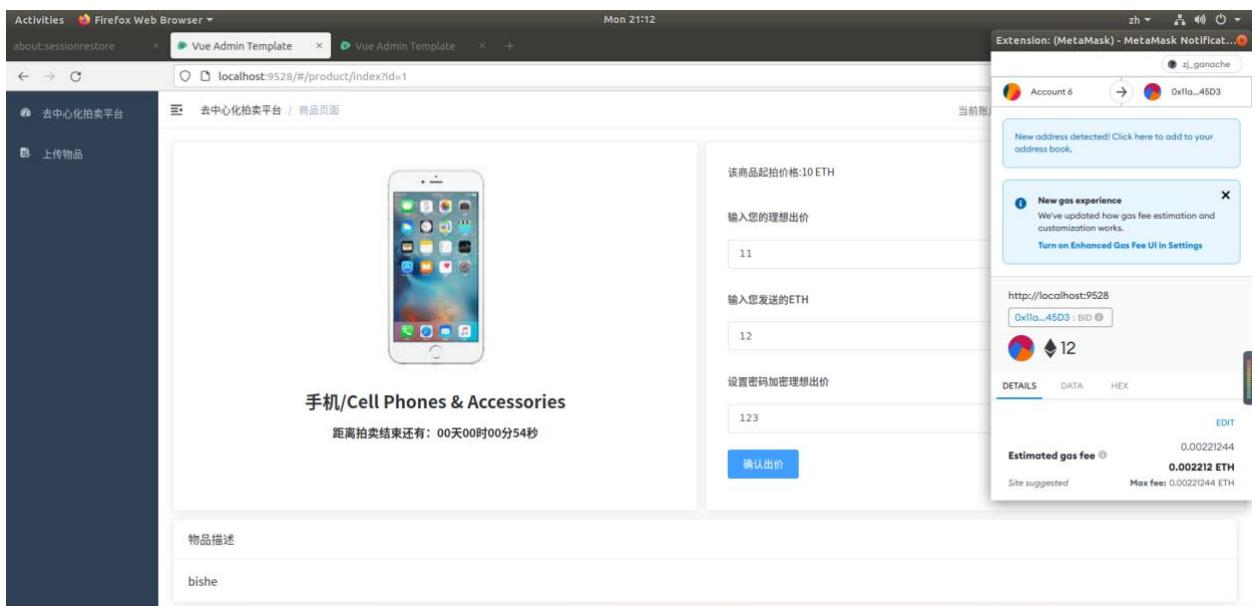
\includegraphics[keepaspectratio,alt={image}]{images/b4984afc162d93bbb214561770783598edb2de6f21a4445fbf4e2d6ef9463b1a.jpg}}

图 4-10 出价页面

用户对商品的揭示出价页面如图 4-11 所示：

\pandocbounded{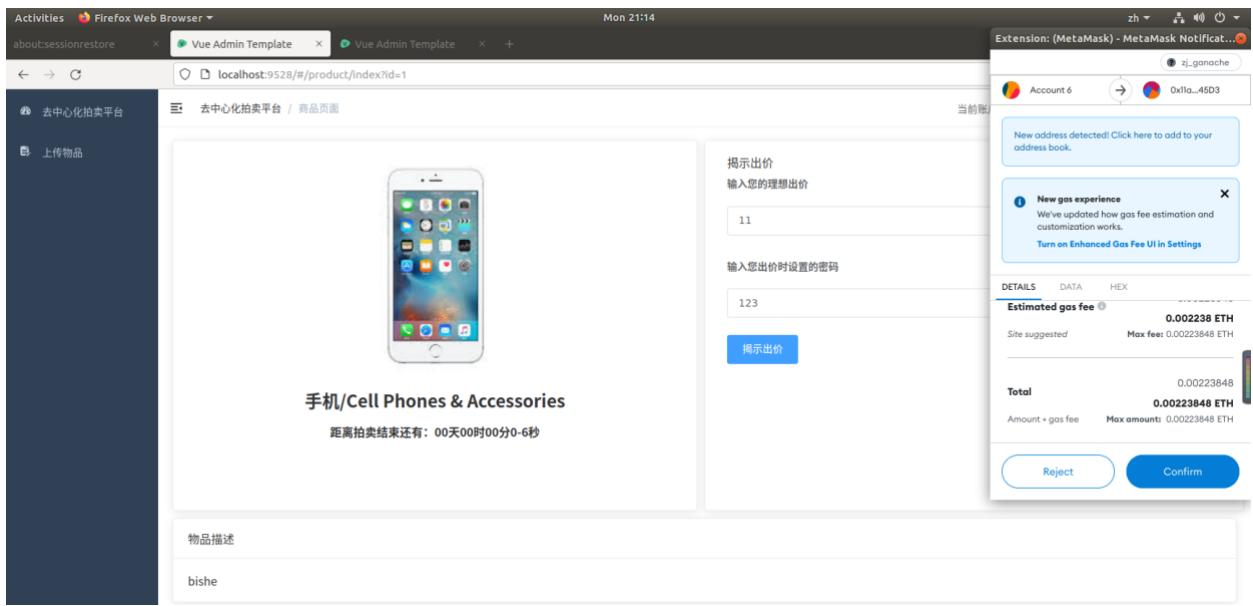
\includegraphics[keepaspectratio,alt={image}]{images/f58954d063b94202e2e8cd9a5cba7ebc7becb69d983195c2d449ce30eae31ca4.jpg}}

图 4-11 揭示出价页面

用户超时揭标页面如图 4-12 所示：

\pandocbounded{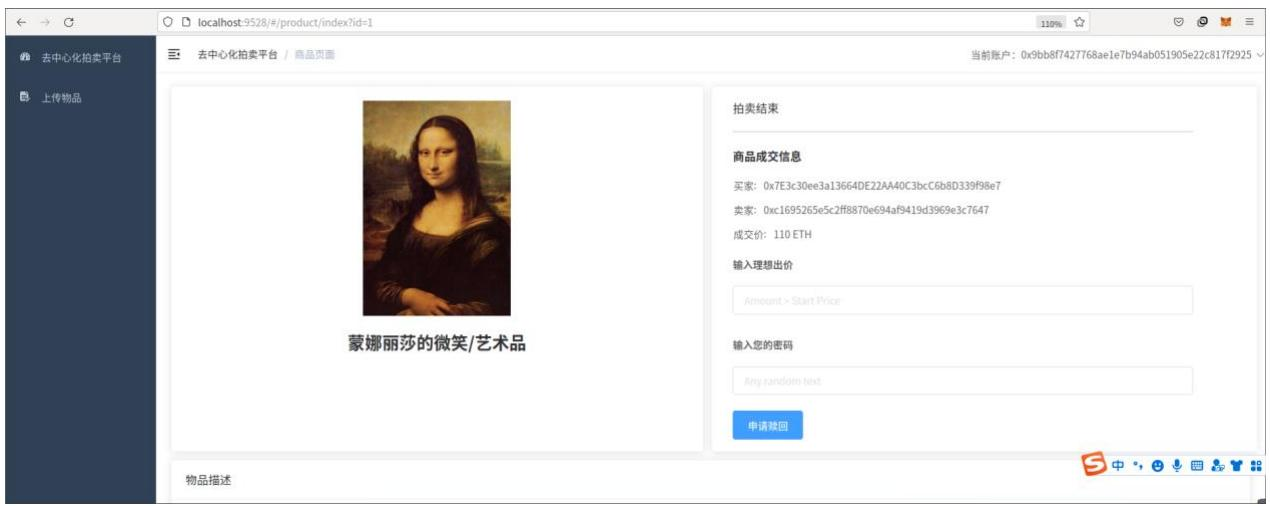
\includegraphics[keepaspectratio,alt={image}]{images/8ba3385651fc0d53f1aa700671c803608c3858e6032ba36a1672137701a009c5.jpg}}

图 4-12 超时揭标页面

无人购买时，商家申请退还押金页面如图 4-13 所示：

\pandocbounded{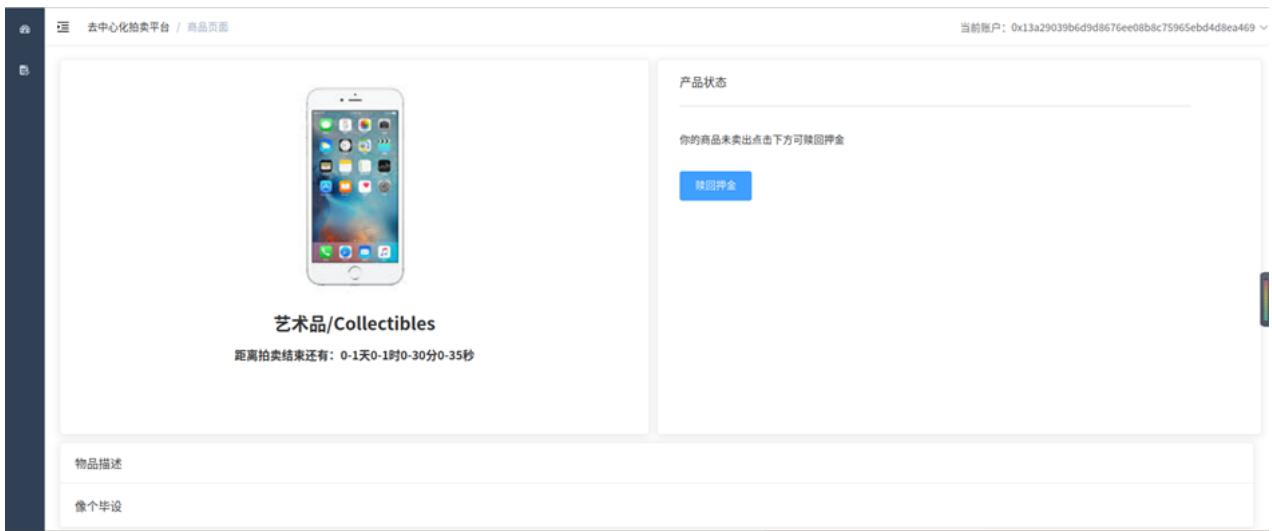
\includegraphics[keepaspectratio,alt={image}]{images/f9eb20d4af7a2984aa00850534abbca3c93f577fd804a6a57bd8fd1284404934.jpg}}

图 4-13 商家申请退还押金页面

\section{4.2.5
资金托管模块}\label{ux8d44ux91d1ux6258ux7ba1ux6a21ux5757-1}

该模块的主要功能通过托管合约 Escrow
来实现，为买卖双方提供了资金保障，并且能够根据买卖双方的操作自动将资金进行付款给对应账户。在拍卖的揭示出价结束后，商品详情页将为买卖双方显示
3个按钮``敲定''、``确认交易''、``申请退款''。

\section{（1）实现过程}\label{ux5b9eux73b0ux8fc7ux7a0b-3}

敲定：买卖双方点击``敲定''即调用 EcommerceStore 合约的
finalizeAuction()函数，首先将判断合约调用者是否为买家或者卖家，然后判断当前时间是否大于拍卖结束时间，

再判断商品的状态是否为拍卖状态，将其状态改变为待交付状态，创建 Escrow
托管合约，将卖家的保证金以及第二高出价发送给托管合约，将第一高出价与第二高出价的差价退还到买家账户。

确认交易：这一功能在托管合约的设计中，我使用了 releaseAmount
键值对、releaseCount
无符号整型来记录买卖双方的确认交易信息。通过在拍卖合约的函数releaseAmountToSeller()内获取托管合约地址内部调用托管合约的同名函数，对买卖双方的操作进行记录，当买卖双方点击``确认交易''之后，托管合约会先判断是否成功完成该商品的交易，再判断拍卖合约调用者是否为该商品的卖家或买家，当第一个人点击时，releaseCount
会增加 1，releaseAmount{[}caller{]}赋值为
true，以便限制每人仅点击一次有效，第二个人再点时，也将进行第一次的记录，但合约还会判断是否是第二个人点击的，如果是，则将买家的付款以及卖家的保证金一并发送给卖家。当双方都完成交易后，将商品拍卖状态修改为已售出。

申请退款：此功能在合约设计中与确认交易类似，但由于卖家或买家申请退款会损失一定的保证金，所以我使用了
refundAmount 键值对、refundCount 无符号整数、firstRefund 地 址 类 型 3
个参数来作为标记，同样通过在拍卖合约的函数refundAmountToBuyer()内获取托管合约地址内部调用托管合约的同名函数，对买卖双方的操作进行记录，当买卖双方点击``申请退款''之后，托管合约会先判断是否成功完成该商品的交易，再判断拍卖合约调用者是否为该商品的卖家或买家，当第一个人点击时，firstRefund
将记录下该地址，refundCount 增加 1，refundAmount{[}caller{]}赋值为
true，第二个点击``申请退款''的，如果第一个点击的人是买家，则将成交价的
\(10 \%\)
发送给卖家作为违约金赔偿，并自动退还卖家保证金；如果第一个点击的人是卖家，则将卖家的保证金以及买家的出价一同发送给买家，卖家将失去保证金。当双方都退款后，将商品拍卖状态修改为未售出。

\section{（2）关键代码}\label{ux5173ux952eux4ee3ux7801-4}

该模块的关键代码主要为合约代码，如代码 4-5 所示。

代码 4-5 资金托管模块合约关键代码

\begin{Shaded}
\begin{Highlighting}[]
\NormalTok{//创建托管  }
\NormalTok{function finalizeAuction(theta\_productId) payable public \{  }
\NormalTok{    address owner = productIdToOwner\_[productId];  }
\NormalTok{    Product storage product = stores[owner][]\_productId];  }
\NormalTok{    address buyer = product.highestBidder;}
\end{Highlighting}
\end{Shaded}

address seller \(=\) owner; //require(msgsender \(\equiv\) seller
\textbar\textbar{} msgsender \(\equiv\) buyer); require(now \(>\)
product.auctionEndTime); require/product.status \(\equiv\)
ProductStatus.Open); product.status \(=\) ProductStatus.Topay; Escrow
escrow \(=\) (new
Escrow).value/product(secondHighestBid.add/product.deposit))(buyer,
seller, product.deposit, product(secondHighestBid);
productToEscrow{[}productsId{]} \(=\) address(escrow);
//退还差价30-20=10，30是理想出价，20是次高 uint refund \(=\)
product.highestBid.sub/product(secondHighestBid); address
uint160(buyer)).transfer(refund); \} //获取托管合约的信息 function
getEscrowInfo(void \_productId) view public returns(address, address,
bool, uint, uint, uint, uint) \{ address escrow \(=\)
productToEscrow{[}productsId{]}; return Escrow(escrow).escrowInfo(); \}
//确认交易接口函数 function releaseAmountToSeller(void \_productId)
payable public \{ address owner \(=\) productIdToOwner{[}productsId{]};
Product storage product \(=\) stores{[}owner{]}{[}productsId{]}; address
escrow \(=\) productToEscrow{[}productsId{]};
Escrow(escrow).releaseAmountToSeller(msgsender);
if(Escrow(escrow).fundsDisbursedShow())\{ product.deposit \(= 0\) . \}
\} //托管合约中确认交易函数 function releaseAmountToSeller(address
caller) payable public \{ require(!fundsDisbursed); if((pager \(\equiv\)
buyer \textbar\textbar{} caller \(\equiv\) seller)\&\& releaseAmount{[}
caller{]} != true)\{ releaseAmount{[} caller{]} \(=\) true; releaseCount
\(=\) releaseCount.add(1); emit UnlockAmount(``release'', caller); \}
if((releaseCount \(\equiv\) 2 \&\& !fundsDisbursed)\textbar\textbar(now
\(>\) createTime.add(24\emph{60}60*30)))\{ address
uint160(seller)).transfer(buyerAmount.add(sellerDesposit));
fundsDisbursed \(=\) true; emit
DisburseAmount(buyerAmount+sellerDesposit, seller); \}

\begin{Shaded}
\begin{Highlighting}[]
\NormalTok{//拍卖合约用户申请退款函数  }
\NormalTok{function refundAmountToBuyer( uint \_productId) payable public \{  }
\NormalTok{    address owner = productIdToOwner\_[productId];  }
\NormalTok{    Product storage product = stores[owner][\_productId];  }
\NormalTok{    address escrow = productToEscrow\_[productId];  }
\NormalTok{    Escrow(escrow).refundAmountToBuyer(msgsender);  }
\NormalTok{    if(Escrow(escrow).fundsDisbursedShow())\{  }
\NormalTok{        product.deposit = 0;  }
\NormalTok{    \}  }
\NormalTok{\}  }
\NormalTok{//托管合约中用户申请退款函数  }
\NormalTok{function refundAmountToBuyer(address caller) payable public \{  }
\NormalTok{    require(!fundsDisbursed);  }
\NormalTok{    if (( caller == seller || caller == buyer) \&\& refundAmount[ caller] != true) \{  }
\NormalTok{        refundAmount[ caller] = true;  }
\NormalTok{        refundCount = refundCount.add(1);  }
\NormalTok{        if (firstRefund == address(0)) \{  }
\NormalTok{            firstRefund = caller;  }
\NormalTok{        \}  }
\NormalTok{        emit UnlockAmount("refund", caller);  }
\NormalTok{    \}  }
\NormalTok{    if (( refundCount == 2 \&\& !fundsDisbursed)||(now \textgreater{} createTime.add(24*60*60*30))) \{  }
\NormalTok{        if (firstRefund == buyer) \{  }
\NormalTok{            address( uint160(buyer)).transfer(buyerAmount.sub(buyerAmount.div(10));  }
\NormalTok{            emit DisburseAmount(buyerAmount.sub(buyerAmount.div(10)), buyer);  }
\NormalTok{        \}  }
\NormalTok{        address( uint160(seller)).transfer(buyerAmount.div(10).add(sellerDesposit));  }
\NormalTok{        emit DisburseAmount(buyerAmount.div(10).add(sellerDesposit), seller);  }
\NormalTok{        fundsDisbursed = true;  }
\NormalTok{    \}  }
\NormalTok{    if (firstRefund == seller) \{  }
\NormalTok{        address( uint160(buyer)).transfer(buyerAmount.add(sellerDesposit));  }
\NormalTok{        emit DisburseAmount(buyerAmount.add(sellerDesposit), buyer);  }
\NormalTok{        fundsDisbursed = true;  }
\NormalTok{    \}  }
\NormalTok{\}}
\end{Highlighting}
\end{Shaded}

\section{（3）界面展示}\label{ux754cux9762ux5c55ux793a-4}

揭标时间结束后，买家与卖家敲定页面，如图
4-14所示，敲定完成后，商品即进入待交付阶段，如图4-15 所示。

\pandocbounded{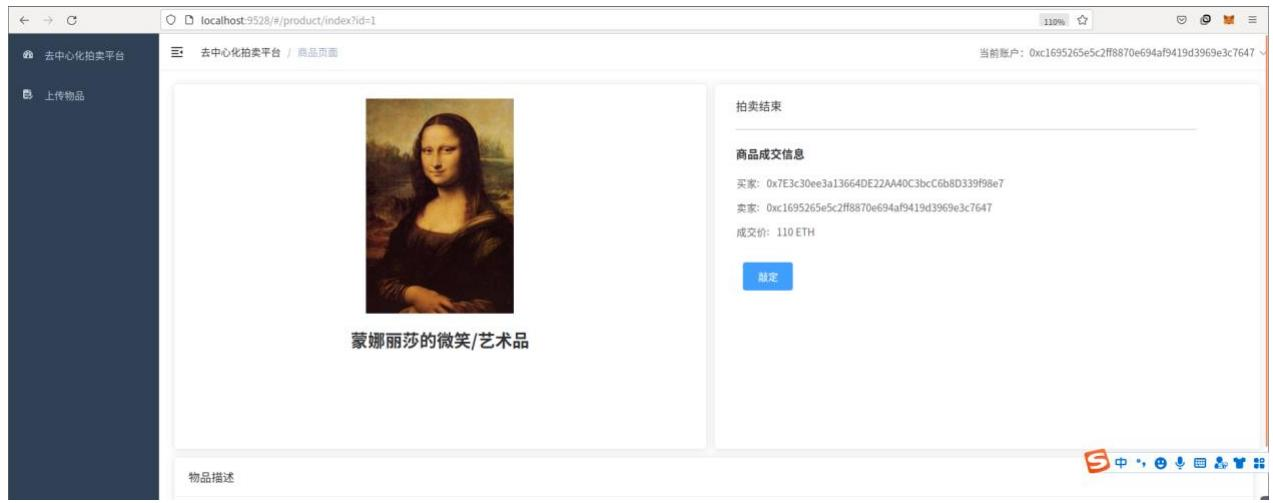
\includegraphics[keepaspectratio,alt={image}]{images/3e4f81da5123a63810efd0dfd177733a41641b781be17c5cad960772869124c2.jpg}}

图 4-14 敲定页面

\pandocbounded{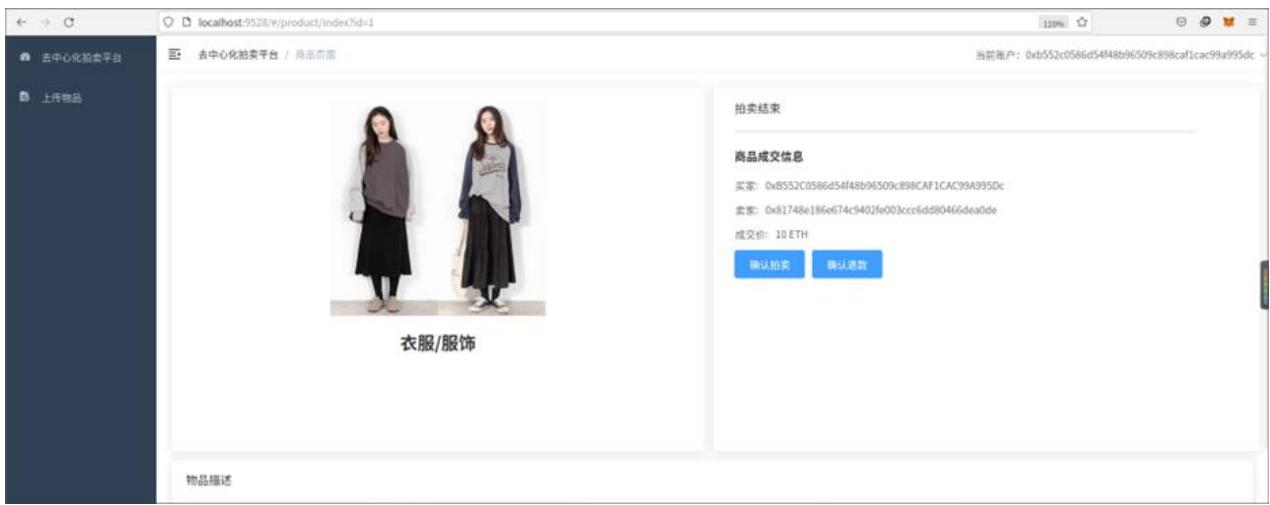
\includegraphics[keepaspectratio,alt={image}]{images/aea674f14e7626e11fe39c13ba720769e9431c8d2f7a712270afcf6e9a7a7638.jpg}}

图 4-15 待交付页面

\section{4.3 非功能模块}\label{ux975eux529fux80fdux6a21ux5757}

本系统所有合约代码中的基本运算均采用 SafeMath
库合约{[}16{]}{[}18{]}{[}19{]}，防止合约被恶意用户的利用溢出漏洞等进行攻击，盗取拍卖合约以及托管合约中的资产。SafeMath
合约代码如代码4-6所示。

代码 4-6 SafeMath 库合约代码

\begin{Shaded}
\begin{Highlighting}[]
\NormalTok{library SafeMath \{}
\NormalTok{//安全乘法函数}
\NormalTok{function mul uint256 a, uint256 b) internal pure returns (uint256) \{}
\NormalTok{    uint256 c = a * b;}
\NormalTok{    require(c / a == b);}
\NormalTok{    return c;}
\NormalTok{\}}
\end{Highlighting}
\end{Shaded}

\begin{Shaded}
\begin{Highlighting}[]
\NormalTok{//安全除法函数  }
\NormalTok{function div( uint256 a, uint256 b) internal pure returns (uint256) \{  }
\NormalTok{    require(b \textgreater{} 0);  }
\NormalTok{    uint256 c = a / b;  }
\NormalTok{    assert(a == b * c + a \% b);  }
\NormalTok{    return c;  }
\NormalTok{\}  }
\NormalTok{//安全减法函数  }
\NormalTok{function sub( uint256 a, uint256 b) internal pure returns (uint256) \{  }
\NormalTok{        require(b \textless{}= a);  }
\NormalTok{        uint256 c = a {-} b;  }
\NormalTok{        return c;  }
\NormalTok{\}  }
\NormalTok{//安全加法函数  }
\NormalTok{function add( uint256 a, uint256 b) internal pure returns (uint256) \{  }
\NormalTok{            uint256 c = a + b;  }
\NormalTok{            require(c \textgreater{}= a);  }
\NormalTok{            return c;  }
\NormalTok{\}  }
\NormalTok{//安全模函数  }
\NormalTok{function mod( uint256 a, uint256 b) internal pure returns (uint256) \{  }
\NormalTok{                require(b != 0);  }
\NormalTok{                return a \% b;  }
\NormalTok{\}}
\end{Highlighting}
\end{Shaded}

\section{4.4 本章小结}\label{ux672cux7ae0ux5c0fux7ed3-3}

本章详细介绍了基于区块链的拍卖平台各个模块的设计以及实现过程，并且展示了部分关键的代码以及前端界面。链接钱包模块主要负责获取用户钱包地址；商品添加模块主要负责把用户输入的商品信息上传到区块链；商品列出及搜索模块主要负责将用户添加的商品从区块链获取并展示到前端界面中；商品拍卖模块主要负责让用户能够对商品出价、揭示出价参与到拍卖；资金托管模块主要负责敲定买卖双方，为买卖双方创建约定。至此开发工作已经收尾，还需后续测试。

\section{第5章
区块链拍卖平台测试}\label{ux7b2c5ux7ae0-ux533aux5757ux94feux62cdux5356ux5e73ux53f0ux6d4bux8bd5}

为了保证平台的稳定可靠，因此对系统进行详细全面的测试，本章将将介绍区块链网络环境，并对系统功能、性能和兼容性三个方面说明测试方法以及展示测试结果。

\section{5.1 Ganache
区块链环境}\label{ganache-ux533aux5757ux94feux73afux5883}

为了方便本系统的开发调试，并没有必要使用真实的公链，本系统选择在本地使用Ganache
搭建以太坊区块链测试环境，并且将区块链的账户信息、交易记录及区块信息等通过图形界面显示出来。Ganache
客户端的以太坊账户信息、区块信息、交易记录分别如图 5-1、图 5-2、图 5-3
所示。

\pandocbounded{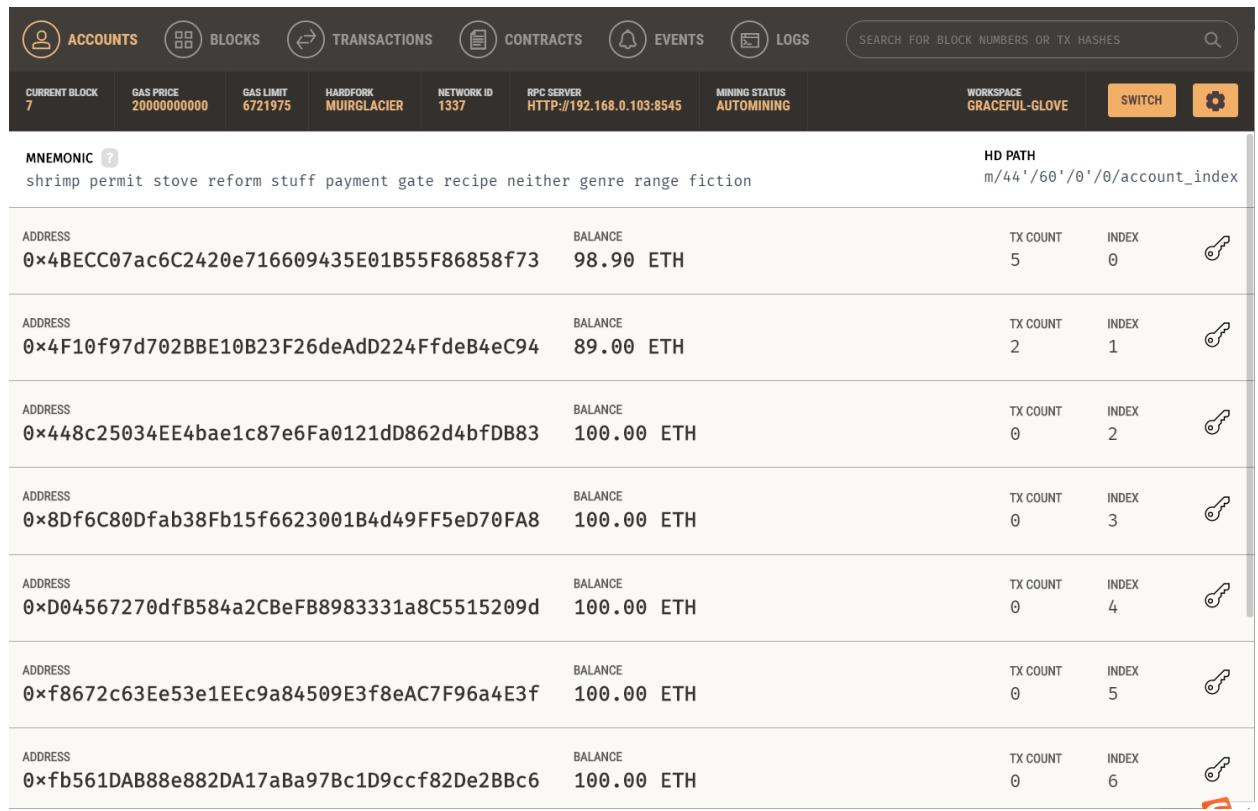
\includegraphics[keepaspectratio,alt={image}]{images/98783614dd3c7d7c264bcc35695be71c10db21fc4549e8a96d9114846cdcf4b5.jpg}}

图 5-1 区块链账户信息

\pandocbounded{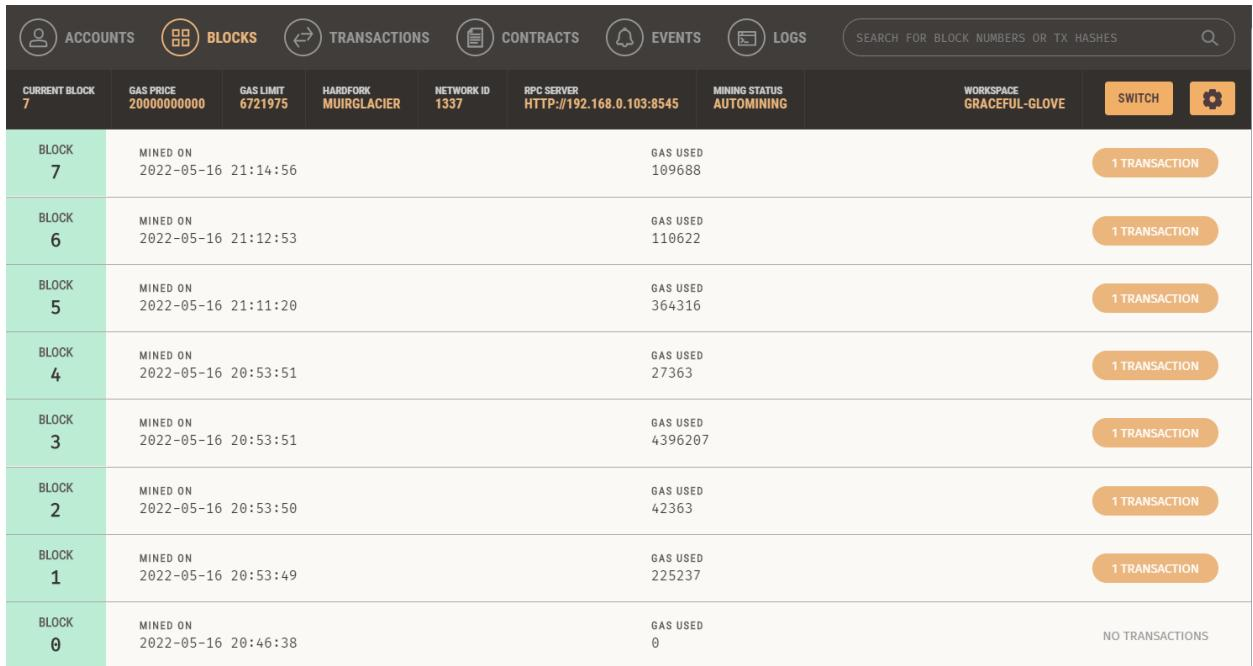
\includegraphics[keepaspectratio,alt={image}]{images/b64b82f99530d6c37b7f602d872c9ab2976496c3a481e8eed0cdd96788219b08.jpg}}

图 5-2 区块链区块信息

\pandocbounded{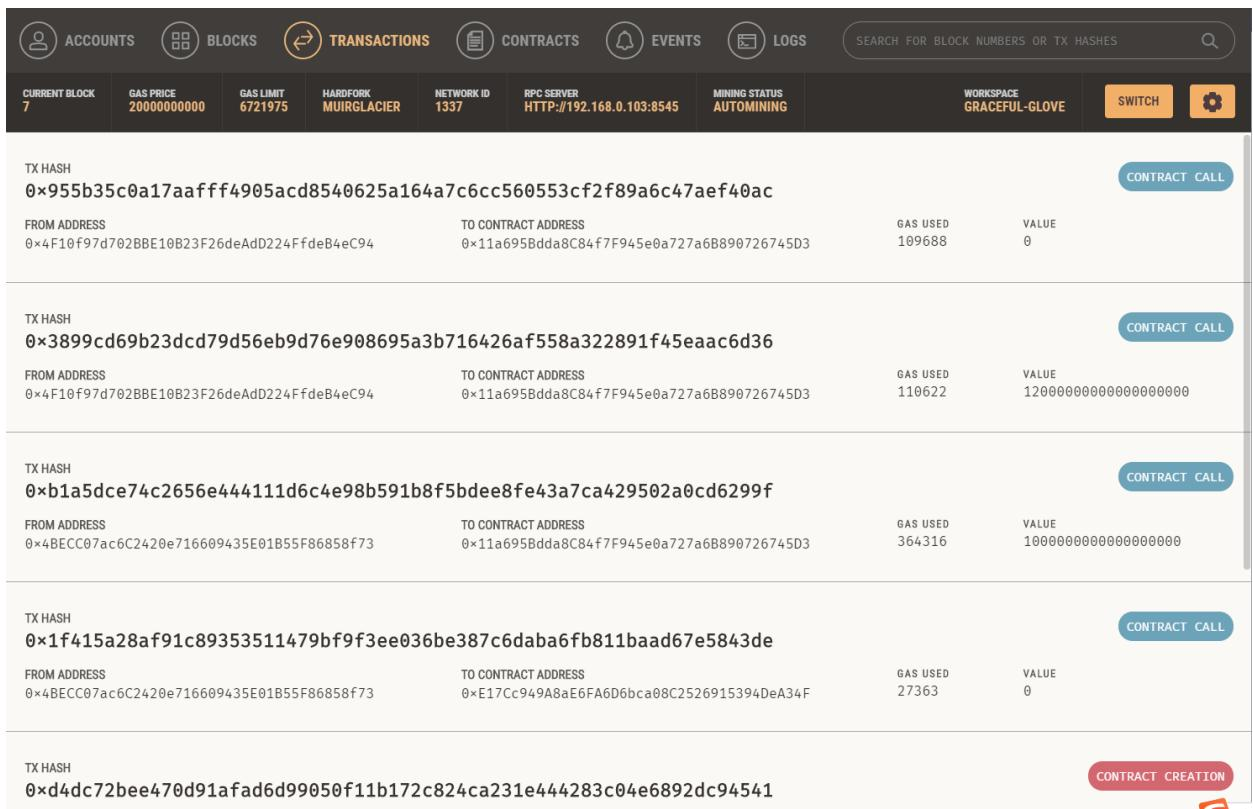
\includegraphics[keepaspectratio,alt={image}]{images/76baa1b9adf776bc8b00c20e3c899caaa0c63f3272c41bb354f5d957893a738a.jpg}}

图 5-3 区块链交易信息

\section{5.2 系统功能测试}\label{ux7cfbux7edfux529fux80fdux6d4bux8bd5}

该项测试主要针对前端与用户交互的功能进行测试，比如添加商品、拍卖出价、拍卖揭价、赎回押金、资金托管等功能，对于拍卖结果是否准确等情况在性能测试中进行。该项测试采用边界值等黑盒测试方法设计并执行
40 个测试用例，表 5-1 列举了部分测试用例。

表 5-1 部分功能测试用例

{\def\LTcaptype{none} % do not increment counter
\begin{longtable}[]{@{}|l|l|l|l|@{}}
\toprule\noalign{}
\endhead
\bottomrule\noalign{}
\endlastfoot
\hline
用例编号 & 操作步骤 & 预期结果 & 实际结果 \\
\hline
case\_01 & 1、用户在钱包链接其他区 块链网路2、进入平台 &
钱包不能链接到网站,网 站不能获取钱包账户 & 钱包不能链接到网站,网
站不能获取钱包账户 \\
\hline
case\_02 & 1、用户在钱包链接 ganache 网络2、进入平台 &
网站可请求钱包链接网 络,用户授权后显示地址 & 网站可请求钱包链接网
络,用户授权后显示地址 \\
\hline
case\_03 & 1、进入商品列表2、点击上 传拍卖物品3、输入商品信
息、上传商品.jpg类型图片 & 上传成功后,可在商品列 表查看 &
上传成功后,可在商品列 表查看 \\
\hline
case\_04 & 1、进入商品列表2、点击上 传拍卖物品3、不选择图片 &
图片为空,上传失败,请 重新上传 & 图片为空,上传失败,请 重新上传 \\
\hline
case\_05 & 1、商品发布者出价阶段进 入该商品的商品详情 &
显示``你的商品正在等待 用户出价中,请等待'' & 显示``你的商品正在等待
用户出价中,请等待'' \\
\hline
case\_06 & 1、商品发布者揭示出价阶 段进入该商品的商品详情 &
显示``你的商品正在揭示 出价中,请等待'' & 显示``你的商品正在揭示
出价中,请等待'' \\
\hline
case\_07 & 1、竞拍者出价阶段进入商 品详情2、输入理想出价、
密码3、点击揭示出价 & 提示揭示出价成功,并能 够得到退还的ETH &
提示揭示出价成功,并能 够得到退还的ETH \\
\hline
case\_08 & 1、竞拍者出价阶段进入商 品详情2、输入理想出价、
错误密码3、点击揭示出价 & 控制台提示 revert错误, 揭示出价失败 &
控制台提示 revert错误, 揭示出价失败 \\
\hline
case\_09 & 1、进入首页2、搜索框中输 入不存在的商品名称 &
页面提示商品未找到 & 页面提示商品未找到 \\
\hline
\end{longtable}
}

续表 5-1 部分功能测试用例

{\def\LTcaptype{none} % do not increment counter
\begin{longtable}[]{@{}|l|l|l|l|@{}}
\toprule\noalign{}
\endhead
\bottomrule\noalign{}
\endlastfoot
\hline
用例编号 & 操作步骤 & 预期结果 & 实际结果 \\
\hline
case\_10 & 1、进入首页2、商品还未开始拍卖，点击商品详情 &
页面提示``商品还未开始拍卖，请等待'' &
页面提示``商品还未开始拍卖，请等待'' \\
\hline
case\_11 & 1、商品揭标结束后，非买卖双方点击商品详情 &
页面正常显示商品的买卖双方地址以及成交价 &
页面正常显示商品的买卖双方地址以及成交价 \\
\hline
case\_12 & 1、商品揭标结束后，买卖双方点击商品详情2、卖家点击敲定 &
页面显示``敲定成功'' & 页面显示``敲定成功'' \\
\hline
case\_13 & 1、敲定后，买卖双方进入商品详情2、买卖双方点击确认交易 &
页面显示``您已完成交易'' & 页面显示``您已完成交易'' \\
\hline
case\_14 & 1、敲定后，买方进入商品详情2、买方点击退款 &
页面显示``您已违约，将扣除您的保证金'' &
页面显示``您已违约，将扣除您的保证金'' \\
\hline
\end{longtable}
}

\section{5.3 系统性能测试}\label{ux7cfbux7edfux6027ux80fdux6d4bux8bd5}

在进行性能测试之前，将对以太坊 Gas
进行简单介绍。交易进入区块需要在一个每个以太坊网络节点都存在的以太坊虚拟机(EVM)中运行计算。而推动计算则需要消耗燃料（Gas）来提供动力。EVM
中的任何操作都会消耗主机的 CPU，磁盘读写，内存。为了维持 EVM
运作，则需要支付手续费购买足够的 Gas
燃料。以太币（ETH）的一个重要用途就是支付交易手续费，而每笔交易的交易手续费并不是固定的。而是根据交易在被矿工收集到区块中时所消耗的资源动态变化的。

为了防止主机``过载''，每个 EVM
操作员都会为执行合约期间消耗的燃料设定上限。因此，如果恶意操作者精心制作了进入无限循环的智能合约，则每个循环都会消耗一些燃料并最终达到极限，此时
EVM
将中止该合约的执行。本质上，合同越大，越复杂，合同执行的操作越多，运行合同的成本就越高。使用燃料价格创建收费市场，允许用户自己决定愿意为每单位的燃料支付多少费用。由于燃料限制，收费市场基本决定挖矿开采什么交易，因为希望获利的矿工会选择费用最高的交易。每笔交易所需要支付的手续费为：燃料消耗量(GasUsed)
* 每单位你愿意支付的单价(GasPrice)。

由于交易时间主要取决于用户所设置的 Gas 价格，时间随 Gas
价格的变化而变化，所以这里没有进行拍卖交易完成的时间测试。主要进行拍卖结果可靠性测试，包括拍卖的出价、揭示出价、商品交易完成的各个阶段，记录不同账户及角色的余额变化情况。

本次测试一共设置
3个账户，一个账户作为商品发布者，即卖家，另外两个账户作为竞拍者，即买家。预设
3 个账户的余额都为 100ETH。由于矿工的 Gas
费用会不定时变化，且占拍卖价格的极少量，所以本测试数据忽略交易产生的旷工
Gas 费用所扣除的ETH对测试结果取整。部分测试数据如表 5-2所示。

表 5-2 拍卖过程余额变化部分测试数据

{\def\LTcaptype{none} % do not increment counter
\begin{longtable}[]{@{}|l|l|l|l|l|l|l|l|@{}}
\toprule\noalign{}
\endhead
\bottomrule\noalign{}
\endlastfoot
\hline
测试用例编号 & 测试操作 & 账户1预 期余额 (ETH) & 账户1测 试余额 (ETH) &
账户2预 期余额 (ETH) & 账户2测 试余额 (ETH) & 账户3预 期余额 (ETH) &
账户3测 试余额 (ETH) \\
\hline
case\_01 & 账户1发布商品,起拍价格定为10ETH & 100-10/10=99 & 99 & 100 &
100 & 100 & 100 \\
\hline
case\_02 & 账户2参与出价:理想出价15ETH,实际发送16ETH & 99 & 99 &
100-16=84 & 84 & 100 & 100 \\
\hline
case\_03 & 账户3参与出价:理想出价16ETH,实际发送20ETH & 99 & 99 & 84 & 84
& 100-20=80 & 80 \\
\hline
case\_04 & 账户2揭示自己的出价 & 99 & 99 & 84+(16-15)=85 & 85 & 80 &
80 \\
\hline
case\_05 & 账户3揭示自己的出价 & 99 & 99 & 85+15=100 & 100 &
80+(20-16)=84 & 84 \\
\hline
case\_06 & 账户3成为该商品的买家,点击``敲定'' & 99 & 99 & 100 & 100 &
84+(16-15)=85 & 85 \\
\hline
\end{longtable}
}

续表 5-2 拍卖过程余额变化部分测试数据

{\def\LTcaptype{none} % do not increment counter
\begin{longtable}[]{@{}|l|l|l|l|l|l|l|l|@{}}
\toprule\noalign{}
\endhead
\bottomrule\noalign{}
\endlastfoot
\hline
测试用例编号 & 测试操作 & 账户1预 期余额 (ETH) & 账户1测 试余额 (ETH) &
账户2预 期余额 (ETH) & 账户2测 试余额 (ETH) & 账户3预 期余额 (ETH) &
账户3测 试余额 (ETH) \\
\hline
case\_07 & 账户3``确认 交付'' & 99 & 99 & 100 & 100 & 85 & 85 \\
\hline
case\_08 & 账户1``确认 交付'' & 99+(15+1) =115 & 115 & 100 & 100 & 85 &
85 \\
\hline
\end{longtable}
}

\section{5.4
系统兼容性测试}\label{ux7cfbux7edfux517cux5bb9ux6027ux6d4bux8bd5}

本系统的后端代码为合约代码，存储在以太坊网络上，只需要安装 MetaMask
钱包插件并链接钱包，即可使用，支持大部分操作系统及浏览器，只要安装了
MetaMask
钱包插件这里对不同的操作系统及浏览器进行兼容性测试，测试结果如表
5-3所示：

表 5-3 兼容性测试情况

{\def\LTcaptype{none} % do not increment counter
\begin{longtable}[]{@{}lllll@{}}
\toprule\noalign{}
\endhead
\bottomrule\noalign{}
\endlastfoot
测试用例编号 & 操作系统 & 浏览器 & 预期结果 & 实际结果 \\
case\_01 & \multirow{3}{*}{Linux ubuntu} & Chrome & 正常使用 &
正常使用 \\
case\_02 & & FireFox & 正常使用 & 正常使用 \\
case\_03 & & IE & 正常使用 & 正常使用 \\
case\_04 & \multirow{3}{*}{Window 10} & Chrome & 正常使用 & 正常使用 \\
case\_05 & & FireFox & 正常使用 & 正常使用 \\
case\_06 & & Safari & 正常使用 & 正常使用 \\
case\_07 & \multirow{2}{*}{MacOS} & Chrome & 正常使用 & 正常使用 \\
case\_08 & & FireFox & 正常使用 & 正常使用 \\
\end{longtable}
}

\section{5.5 本章小结}\label{ux672cux7ae0ux5c0fux7ed3-4}

本章主要是对已开发完成的系统的区块链环境做了简要介绍，对系统的各个功能测试、商品拍卖的整个流程的功能实现结果的正确可靠性的测试以及兼容性测试。测试结果表明，本系统的设计与实现达到预期效果，可以准确安全的实现基于区块链的维克里拍卖并稳定使用。

\section{结论}\label{ux7ed3ux8bba}

本文分析了在目前的互联网时代背景下，保证拍卖过程中的个人隐私、资产安全和降低商业成本的重要性，结合国内外的拍卖平台和区块链+IPFS
的应用的研究现状阐述了现有的线下与线上拍卖平台的优势与不足，提出了基于区块链的拍卖平台。

本文首先介绍了本系统相关理论知识与关键技术：维克里拍卖的原理、区块链的概念特点及分类、以太坊概念及特点、IPFS
的概念及优势以及智能合约的相关知识。然后对系统进行了需求分析，介绍了本平台是一个去中心化的点对点拍卖平台并根据不同角色不同功能需求，对系统用例以及主要功能进行了简要的描述，并作出系统概要设计。

其次，对该系统的详细代码设计与实现过程进行了描述，将系统在概要设计中分成的链接钱包、商品添加、商品列出与搜索、商品拍卖、资金托管五个模块给出了设计思路以及实现效果。系统的所有功能的实现均需要用户用自己的
MetaMask
钱包账户的私钥对交易进行签名确认，这保证了用户在使用平台的过程中较高的安全性，商品添加时，使用
IPFS 技术，将大文件存储在 IPFS 网络上，再将其 Hash
通过以太坊智能合约存储在以太坊区块链上，拍卖方式使用维克里拍卖，使用
sha256加密函数对用户拍卖理想出价进行加密运算后存储在以太坊区块链上，拍卖过程中的核心功能均通过调用以太坊智能合约实现。最后对系统进行了较为全面的测试，表现出本平台拍卖流程的功能较为完善、运行稳定、拍卖结果准确可靠，达到既定的预期目标。

本平台与目前市面上的中心化拍卖平台相比，在拍卖过程的安全、可信程度上确实比较有优势，商品发布者也不需要给任何人支付交易佣金，同时本平台采用经过改进后的维克里拍卖机制，能够在用户忘记揭标的情况下，对用户的资产进行退回，总的来说无论是对于商家还是竞拍者都是更加友好、公平的。

但是，本平台仍存在一些不足之处，需要在以后的工作中进一步改进与完善，主要有以下内容：

（1）本平台暂未开发实现用户之间相互查看购买和销售记录以及交易完成后的评价功能，还需完善这些功能。

（2）本平台在对于报错提示上还不够完善，存在一些前端页面的报错提示未实现，后续需要针对每一种报错给用户带来更加直观的提示消息。

（3）目前本平台只能处理拍卖交易的链上完成部分，并不能真正联系到实物，所以还需要将物流信息上链，进一步撮合交易的完成。

\section{致谢}\label{ux81f4ux8c22}

时光飞逝，转眼间，大学生涯即将结束，在本篇论文即将收尾之时，我要衷心的感谢所有在这过程中关心和帮助过我的人。

首先，谨向我的指导老师孙海峰老师说一声谢谢！感谢您这些天来对我的毕设的指导与建议。当我设计过程中遇到了一些不可解决的问题时，孙老师总是能为我答疑解惑。从毕业设计到毕业论文，从整体方向到细节思路，孙老师都给予了我充分的沟通和指导建议。同时还要感谢听我开题答辩的老师们，她们首先指出了我在开题报告中的一些错误的设计思路准确，经过我对老师们的意见进行深思以及各方资料的查阅，让我有机会对本系统的错误思想进行整改。其次，感谢我在实习公司的领导及同事，耐心地给我讲解区块链智能合约开发以及漏洞的防护相关知识以及处理开发过程中遇到的一些报错问题，让我少走了许多弯路。

最后，感谢曾经教育和帮助我的所有老师以及为我评阅本论文而付出辛勤劳动的各位老师。

\section{参考文献}\label{ux53c2ux8003ux6587ux732e}

{[}1{]}易衷平. 基于区块链+IPFS
的在线拍卖平台实现{[}D{]}.浙江工商大学,2020.

{[}2{]}姚前.区块链技术十周年:回眸与前瞻{[}J{]}.当代金融家,2019(01):92-95.

{[}3{]}张鹏.区块链技术在档案信息化建设中的应用研究{[}J{]}.城建档案,2020(11):18-19.

{[}4{]}范硕,宋波,董旭德,韩天齐.基于区块链的药品溯源追踪方案研究设计{[}J{]}.成都信息工程大学学报,2019,34(3):267-273.

{[}5{]}冯琳琳,司博章,许亨哲.基于区块链的危化品追溯管理系统{[}J{]}.科技创新与应用,2021(6):185-187.

{[}6{]}张怀印,凌宗亮.区块链技术在商标领域的证明作用{[}J{]}.知识产权,2018(05):76-82.

{[}7{]}孙士奇.区块链技术的发展及应用{[}J{]}.信息系统工程,2018(10):85-86+88.

{[}8{]}郭超.区块链在中国银行山东省分行的应用模式研究{[}D{]}.山东大学,2020.

{[}9{]}曲晓丽.防止网上假名报价的几种拍卖机制的比较{[}D{]}.对外经济贸易大学,2003.

{[}10{]}付金华.
高效能区块链关键技术及应用研究{[}D{]}.战略支援部队信息工程大学,2020.

{[}11{]}易勤,欧嵬,刘威等.基于区块链的慈善系统的研究与实现{[}J{]}.计算机时代,2020(2):62-66.

{[}12{]}陈巧萍.区块链发展下农产品跨境电商的良性生态系统构建{[}J{]}.农业经济,2021(10):132-134.

{[}13{]}严正. 分布式电商系统移动端的设计与实现{[}D{]}.北京邮电大学,2020.

{[}14{]}王明生,曹鹤阳,李佩瑶.基于区块链的去中心化信贷系统及应用{[}J{]}.通信学报,2019,40(8):169-177.

{[}15{]}王升,范思宇,杜玉洁等.基于区块链技术的文档防篡改系统{[}J{]}.网络安全技术与应用,2021(2):31-32.

{[}16{]}倪远东,张超,殷婷婷.智能合约安全漏洞研究综述{[}J{]}.信息安全学报,2020,5(3):78-99.

{[}17{]}Fujita, Satoshi.Similarity Search in InterPlanetary File System
with the Aid of Locality Sensitive Hash{[}J{]}.I E I C E Transactions on
Information and Systems, 2021, E104D(10):1616-1623.

{[}18{]}Szabo N.Formalizing and securing relationships on public
networks{[}EB/OL{]}.{[}2020-09-
10{]}.https://firstmonday.org/ojs/index.php/fm/article/view/548.

{[}19{]}Giordano F, Bachfischer A, Carder G, et al.~OpenZeppelin is a
library for secure smartcontract
development{[}EB/OL{]}.{[}2020-09-10{]}.https://github.com/
OpenZeppelin/openzeppelin-contracts.

{[}20{]}Naz, Muqaddas 等 .A Secure Data Sharing Platform Using
Blockchain and Interplanetary FileSystem{[}J{]}.SUSTAINABILITY,2019,
11(24).

{[}21{]}Xumin, Huang, Dongdong 等.Securing Parked Vehicle Assisted Fog
Computing With Blockchain andOptimal Smart Contract
Design{[}J{]}.自动化学报：英文版, 2020, 7(2):426-441.

\end{document}
